% !TEX root = presentation.tex
% !BIB program = biber
% !TEX program = xelatex


\documentclass[aspectratio=169,xetex]{beamer}

% Default packages
\usepackage[T1]{fontenc}
\usepackage[utf8]{inputenc}
\usepackage[english]{babel}
\usepackage{csquotes}
\usepackage{booktabs}
\usepackage{siunitx}
\usepackage{multicol}
\usepackage{caption}
\usepackage{subcaption}

\usepackage[
    % backend=biber,
    % style=numeric,
    % sorting=ynt
    backend=biber,
    natbib=true, 
    style=numeric,
    abbreviate=false,
    dateabbrev=false,
    maxbibnames=14,
    urldate=long,
    date=year,
    url=false,
    backref=true,
    sortcites
]{biblatex}
\addbibresource{../bibliography/zotero-references.bib}
\setbeamertemplate{bibliography item}{\insertbiblabel}

\usepackage{multicol}
\usepackage{multirow}
\usepackage{makecell}
\usepackage{booktabs}
\usepackage{enumerate}
% \usepackage{enumitem}
\usepackage{adjustbox}
\usepackage{siunitx}
\usepackage{tabularx,colortbl}

\usepackage{pgfplots}
\pgfplotsset{compat=1.17}
\usepgfplotslibrary{fillbetween}
\pgfmathdeclarefunction{gauss}{2}
    {\pgfmathparse{1/(#2*sqrt(2*pi))*exp(-((x-#1)^2)/(2*#2^2))}}

% Colors
\usepackage{xcolor}
\definecolor{Blue}{rgb}{0.0,0.0,1.0}
\definecolor{Red}{rgb}{1.0,0.0,0.0}

% Load preamble from thesis
\definecolor{customgreen} {RGB}{217	234	212}
\definecolor{customblue}  {RGB}{205	226	242}
\definecolor{custommorered}{RGB}{218 46 42}
\definecolor{customred}{RGB}{255 182 173}%{255 149 150}

\definecolor{presentation_green_shaded}{RGB}{217 234 211}
\definecolor{presentation_green}{RGB}{197 228 186}
\definecolor{presentation_blue_shaded}{RGB}{201 218 248}
\definecolor{presentation_blue}{RGB}{180 205 248}
\definecolor{presentation_orange}{RGB}{255 219 182}
\definecolor{presentation_orange_shaded}{RGB}{252 229 205}
\definecolor{presentation_red}{RGB}{255 182 173}
\definecolor{presentation_red_shaded}{RGB}{249 228 228}

\colorlet{observed-color}{customgreen}
\colorlet{latent-color}{customblue}
\colorlet{deterministic-color}{gray!15}
\colorlet{deterministic-skip-color}{custommorered}
\colorlet{shared-function-color}{blue}

\definecolor{theme-green}{RGB}{41 114 114}

% Checkmark and cross for brief overview paper
\usepackage{pifont}
\definecolor{ForestGreen}{RGB}{34,139,34}
\definecolor{xred}{HTML}{C91E12}
\definecolor{xorange}{RGB}{230,145,56}
\newcommand{\cmark}{{\color{ForestGreen}\ding{51}}}%
\newcommand{\xmark}{{\color{xred}\ding{55}}}%
\newcommand{\xmarkshaded}{{\color{xorange}\ding{55}}}%

    
% TikZ
\usepackage{tikz}
\usetikzlibrary{
    arrows,
    backgrounds,
    matrix,
    positioning,
    shapes,
    shapes.multipart,
    topaths,
    bayesnet,
}
\tikzset{
state/.style={
       rectangle split,
       rectangle split parts=2,
       rectangle split part fill={red!30,blue!20},
       rounded corners,
       draw=black, very thick,
       minimum height=2em,
       text width=3cm,
       inner sep=2pt,
       text centered,
       }
}
\usepackage[beamer,customcolors]{hf-tikz}
\tikzset{hl/.style={
    set fill color=presentation_green_shaded,%red!80!black!40,
    set border color=presentation_green_shaded,
  },
}

\setbeamertemplate{caption}[numbered]


%!TEX root = ../thesis.tex

% Math symbols
% \usepackage{amsmath}
% \usepackage{amssymb}

% Text fonts (http://www.macfreek.nl/memory/Fonts_in_LaTeX)
% Install fonts from /usr/local/texlive/<version>/texmf-dist/fonts/opentype/public
% \usepackage[utf8]{inputenc}
\usepackage{fontspec}
% \usepackage[T1]{fontenc}
% \usepackage{lmodern}
\usepackage{slantsc}
% \RequirePackage{fix-cm}
\usepackage{bold-extra}
\usepackage{csquotes}       % language sensitive quotation facilities


% Method that works with TeXLive 2023
% \usepackage[math-style=upright]{unicode-math}
% \setmainfont{texgyrepagella-regular.otf}[Scale=1.0, Ligatures={Common,Rare,TeX}]  % Or Palatino Linotype, etc.
% \setmathfont{texgyrepagella-math.otf}[Scale=MatchLowercase]
% \setmathfont{euler.otf}[range={up/{Latin,latin,Greek,Greek}, bfup/{Latin,latin,Greek,Greek}, cal, bfcal, frak, bffrak}, Scale=MatchLowercase, script-features={}, sscript-features={}]


% Method that works with TeXLive 2023 and is simpler and has fewer missing characters
\usepackage{newpxtext, eulerpx}


% Method that should be best practice for TeXLive
% These packages were recommended but seem to cause trouble with the euler-math and unicode-math packages.
% \usepackage{newpxtext,newpxmath}
% \setmainfont{texgyrepagella-regular.otf}[Scale=1.0, Ligatures={Common,Rare,TeX}]  % Or Palatino Linotype, etc.
% \usepackage{euler-math}


% Method that works with TeXLive 2022 (but is missing some special characters e.g. ê, ç)
% \usepackage{amssymb}
% \usepackage{upgreek}
% \usepackage{mathpazo}
% \usepackage[OT1,euler-digits]{eulervm}
% \renewcommand{\mathbf}{\mathbold}  % euler requires \mathbold for bold math





% % Remove: "Font shape `T1/eulervm/m/n' undefined (Font) using `T1/cmr/m/n' instead."
% \usepackage{substitutefont}
% \substitutefont{TS1}{eulervm}{cmr}

%
% [
%   Extension=.otf,
%   UprightFont=*-regular,
%   ItalicFont=*-italic,
%   BoldFont=*-bold,
%   BoldItalicFont=*-bolditalic,
%   BoldSmallCapsFont=*-boldsmallcaps,
%   Numbers=OldStyle,
% ]

% \setmainfont{QTPalatine}

% \DeclareCharacterInheritance
%    { encoding = {TU,EU1,EU2},
%      family   = {QTPalatine} }
%    { A = {\`A,\'A,\^A,\~A,\"A,\r A},
%      a = {\`a,\'a,\^a,\~a,\"a,\r a},
%      C = {\c C},
%      c = {\c c},
%      D = {\DH},
%      d = {\dj},
%      E = {\`E,\'E,\^E,\"E},
%      e = {\`e,\'e,\^e,\"e},
%      I = {\`I,\'I,\^I,\"I},
%      i = {\`i,\'i,\^i,\"i,\i},
%      L = {\L},
%      l = {\l},
%      N = {\~N},
%      n = {\~n},
%      O = {\O,\`O,\'O,\^O,\~O,\"O},
%      o = {\o,\`o,\'o,\^o,\~o,\"o},
%      S = {\v S},
%      s = {\v s},
%      U = {\`U,\'U,\^U,\"U},
%      u = {\`u,\'u,\^u,\"u},
%      Y = {\'Y,\"Y},
%      y = {\'y,\"y},
%      Z = {\v Z},
%      z = {\v z}
%    }


% % Sans-serif font
% \setsansfont[
%     Ligatures=TeX,
%     Extension=.otf,
%     UprightFont=*-regular,
%     BoldFont=*-bold,
%     ItalicFont=*-italic,
%     BoldItalicFont=*-bolditalic,
%     % SlantedFont=,
%     % BoldSlantedFont=,
%     % SmallCapsFont=
%     Scale=0.8      % Adjustmens when using math in sections
% ]{texgyreadventor}


% Monospaced
% \setmonofont[Scale=MatchLowercase]{Linux Biolinum O}

%\setsansfont[Ligatures=TeX]{Neo Sans Intel}    % Neo Sans Intel – Like DTU font but more symbols
%\setsansfont[
%    Ligatures=TeX,
%    Scale=0.8
%]{NeoSans}           % NeoSans – DTU font (missing `+' symbols and other)
% \setsansfont[Ligatures=TeX]{CMU Sans Serif}    % Computer Modern Unicode font
%\setsansfont[Ligatures=TeX]{Latin Modern Sans} % Latin Modern Sans serif font

% Use this for more convienent sans serif font in math mode.
%\setmathsf{Latin Modern Sans}

\input{../preamble/bayesnet_extras}
% \input{../preamble/etc.tex}
\input{../preamble/dtucolors.sty}
%!TEX root = ../thesis.tex

% This information is used in titlepage, colophon, preface and hyperref setup (pdf metainfo), and other options.

%\def\thesistypeabbr{B.Eng.}
%\def\thesistype    {Bachelor of Engineering}
%\def\thesistypeabbr{B.Sc.Eng.}
%\def\thesistype    {Bachelor of Science in Engineering}
%\def\thesistypeabbr{M.Sc.}
%\def\thesistype    {Master of Science in Engineering}
\def\thesistypeabbr{Ph.D.}
\def\thesistype    {Doctor of Philosophy}

\def\thesisdepshort{DTU Compute}
\def\thesisdep     {Department of Applied Mathematics and Computer Science}

\def\thesisauthor  {Jakob Drachmann Havtorn}
\def\thesistitle   {Uncertainty Estimation for Machine Learning Systems}
\def\thesissubtitle{Self-assessment on Medical Conversations}
\def\thesislocation{Copenhagen}
\def\thesisyear    {2023}
\def\thesismonth   {August}
\def\thesisday     {31}

\def\papersize     {b5paper} % Final papersize (b5paper/a4paper), recommended papersize for DTU Compute is b5paper
\def\showtrims     {false}   % Print on larger paper than \papersize and show trim marks (true/false)?
\def\showframe     {false}   % Show frame of writeable area, marginparsep and marginpar (true/false)?

\def\showtodos     {true}    % Show todos (true/false)?
\def\confidential  {false}   % Confidential thesis (true/false)?


%!TEX root = ../Thesis.tex

% Parenthesis
\providecommand{\pa}[1]{{\left(#1\right)}}
  \renewcommand{\pa}[1]{{\left(#1\right)}}
\providecommand{\bra}[1]{{\left[#1\right]}}
  \renewcommand{\bra}[1]{{\left[#1\right]}}
\providecommand{\cbra}[1]{{\left\{#1\right\}}}
  \renewcommand{\cbra}[1]{{\left\{#1\right\}}}
\providecommand{\vbra}[1]{{\left\langle#1\right\rangle}}
  \renewcommand{\vbra}[1]{{\left\langle#1\right\rangle}}

% Matrices for displayed expressions
\providecommand{\mat}[1]{{\begin{matrix}#1\end{matrix}}}
  \renewcommand{\mat}[1]{{\begin{matrix}#1\end{matrix}}}
\providecommand{\pmat}[1]{{\begin{pmatrix}#1\end{pmatrix}}}
  \renewcommand{\pmat}[1]{{\begin{pmatrix}#1\end{pmatrix}}}
\providecommand{\bmat}[1]{{\begin{bmatrix}#1\end{bmatrix}}}
  \renewcommand{\bmat}[1]{{\begin{bmatrix}#1\end{bmatrix}}}

% Variations of \frac and \sfrac
\providecommand{\pfrac}[2]{{\left(\frac{#1}{#2}\right)}}
  \renewcommand{\pfrac}[2]{{\left(\frac{#1}{#2}\right)}}
\providecommand{\bfrac}[2]{{\left[\frac{#1}{#2}\right]}}
  \renewcommand{\bfrac}[2]{{\left[\frac{#1}{#2}\right]}}
\providecommand{\psfrac}[2]{{\left(\sfrac{#1}{#2}\right)}}
  \renewcommand{\psfrac}[2]{{\left(\sfrac{#1}{#2}\right)}}
\providecommand{\bsfrac}[2]{{\left[\sfrac{#1}{#2}\right]}}
  \renewcommand{\bsfrac}[2]{{\left[\sfrac{#1}{#2}\right]}}

% for small matrices to be used in in-line expressions
\providecommand{\sm}[1]{{\left\{#1\right\}}}
  \renewcommand{\sm}[1]{{\left\{#1\right\}}}
\providecommand{\psm}[1]{{\pa{\sm{#1}}}}
  \renewcommand{\psm}[1]{{\pa{\sm{#1}}}}
\providecommand{\bsm}[1]{{\bra{\sm{#1}}}}
  \renewcommand{\bsm}[1]{{\bra{\sm{#1}}}}

% Norm
\providecommand{\norm}[1]{{\left\lVert#1\right\rVert}}
  \renewcommand{\norm}[1]{{\left\lVert#1\right\rVert}}
% Size
\providecommand{\size}[1]{{\left\lvert#1\right\rvert}}
  \renewcommand{\size}[1]{{\left\lvert#1\right\rvert}}
% Trace
\providecommand{\Tr}[1]{{\text{Tr}\left[#1\right]}}
  \renewcommand{\Tr}[1]{{\text{Tr}\left[#1\right]}}
% Tranpose
\providecommand{\transpose}{{^\mathrm{T}}}
  \renewcommand{\transpose}{{^\mathrm{T}}}

% Derivatives
\providecommand{\od}[3][]{{\frac{\text{d}^{#1}#2}{\text{d}^{#1}#3}}}
  \renewcommand{\od}[3][]{{\frac{\text{d}^{#1}#2}{\text{d}^{#1}#3}}}
\providecommand{\pd}[3][]{{\frac{\partial^{#1}#2}{\partial^{#1}#3}}}
  \renewcommand{\pd}[3][]{{\frac{\partial^{#1}#2}{\partial^{#1}#3}}}

% Bold upright letters
\providecommand{\a}{{\mathbf{a}}}
  \renewcommand{\a}{{\mathbf{a}}}
\providecommand{\b}{{\mathbf{b}}}
  \renewcommand{\b}{{\mathbf{b}}}
\providecommand{\c}{{\mathbf{c}}}
  \renewcommand{\c}{{\mathbf{c}}}
\providecommand{\d}{{\mathbf{d}}}
  \renewcommand{\d}{{\mathbf{d}}}
\providecommand{\e}{{\mathbf{e}}}
  \renewcommand{\e}{{\mathbf{e}}}
\providecommand{\f}{{\mathbf{f}}}
  \renewcommand{\f}{{\mathbf{f}}}
\providecommand{\g}{{\mathbf{g}}}
  \renewcommand{\g}{{\mathbf{g}}}
\providecommand{\h}{{\mathbf{h}}}
  \renewcommand{\h}{{\mathbf{h}}}
\providecommand{\i}{{\mathbf{i}}}
  \renewcommand{\i}{{\mathbf{i}}}
\providecommand{\j}{{\mathbf{j}}}
  \renewcommand{\j}{{\mathbf{j}}}
\providecommand{\k}{{\mathbf{k}}}
  \renewcommand{\k}{{\mathbf{k}}}
\providecommand{\l}{{\mathbf{l}}}
  \renewcommand{\l}{{\mathbf{l}}}
\providecommand{\m}{{\mathbf{m}}}
  \renewcommand{\m}{{\mathbf{m}}}
\providecommand{\n}{{\mathbf{n}}}
  \renewcommand{\n}{{\mathbf{n}}}
\providecommand{\o}{{\mathbf{o}}}
  \renewcommand{\o}{{\mathbf{o}}}
\providecommand{\p}{{\mathbf{p}}}
  \renewcommand{\p}{{\mathbf{p}}}
\providecommand{\q}{{\mathbf{q}}}
  \renewcommand{\q}{{\mathbf{q}}}
\providecommand{\r}{{\mathbf{r}}}
  \renewcommand{\r}{{\mathbf{r}}}
\providecommand{\s}{{\mathbf{s}}}
  \renewcommand{\s}{{\mathbf{s}}}
\providecommand{\t}{{\mathbf{t}}}
  \renewcommand{\t}{{\mathbf{t}}}
\providecommand{\u}{{\mathbf{u}}}
  \renewcommand{\u}{{\mathbf{u}}}
\providecommand{\v}{{\mathbf{v}}}
  \renewcommand{\v}{{\mathbf{v}}}
\providecommand{\w}{{\mathbf{w}}}
  \renewcommand{\w}{{\mathbf{w}}}
\providecommand{\x}{{\mathbf{x}}}
  \renewcommand{\x}{{\mathbf{x}}}
\providecommand{\y}{{\mathbf{y}}}
  \renewcommand{\y}{{\mathbf{y}}}
\providecommand{\z}{{\mathbf{z}}}
  \renewcommand{\z}{{\mathbf{z}}}
\providecommand{\A}{{\mathbf{A}}}
  \renewcommand{\A}{{\mathbf{A}}}
\providecommand{\B}{{\mathbf{B}}}
  \renewcommand{\B}{{\mathbf{B}}}
\providecommand{\C}{{\mathbf{C}}}
  \renewcommand{\C}{{\mathbf{C}}}
\providecommand{\D}{{\mathbf{D}}}
  \renewcommand{\D}{{\mathbf{D}}}
\providecommand{\E}{{\mathbf{E}}}
  \renewcommand{\E}{{\mathbf{E}}}
\providecommand{\F}{{\mathbf{F}}}
  \renewcommand{\F}{{\mathbf{F}}}
\providecommand{\G}{{\mathbf{G}}}
  \renewcommand{\G}{{\mathbf{G}}}
\providecommand{\H}{{\mathbf{H}}}
  \renewcommand{\H}{{\mathbf{H}}}
\providecommand{\I}{{\mathbf{I}}}
  \renewcommand{\I}{{\mathbf{I}}}
\providecommand{\J}{{\mathbf{J}}}
  \renewcommand{\J}{{\mathbf{J}}}
\providecommand{\K}{{\mathbf{K}}}
  \renewcommand{\K}{{\mathbf{K}}}
\providecommand{\L}{{\mathbf{L}}}
  \renewcommand{\L}{{\mathbf{L}}}
\providecommand{\M}{{\mathbf{M}}}
  \renewcommand{\M}{{\mathbf{M}}}
\providecommand{\N}{{\mathbf{N}}}
  \renewcommand{\N}{{\mathbf{N}}}
\providecommand{\O}{{\mathbf{O}}}
  \renewcommand{\O}{{\mathbf{O}}}
\providecommand{\P}{{\mathbf{P}}}
  \renewcommand{\P}{{\mathbf{P}}}
\providecommand{\Q}{{\mathbf{Q}}}
  \renewcommand{\Q}{{\mathbf{Q}}}
\providecommand{\R}{{\mathbf{R}}}
  \renewcommand{\R}{{\mathbf{R}}}
\providecommand{\S}{{\mathbf{S}}}
  \renewcommand{\S}{{\mathbf{S}}}
\providecommand{\T}{{\mathbf{T}}}
  \renewcommand{\T}{{\mathbf{T}}}
\providecommand{\U}{{\mathbf{U}}}
  \renewcommand{\U}{{\mathbf{U}}}
\providecommand{\V}{{\mathbf{V}}}
  \renewcommand{\V}{{\mathbf{V}}}
\providecommand{\W}{{\mathbf{W}}}
  \renewcommand{\W}{{\mathbf{W}}}
\providecommand{\X}{{\mathbf{X}}}
  \renewcommand{\X}{{\mathbf{X}}}
\providecommand{\Y}{{\mathbf{Y}}}
  \renewcommand{\Y}{{\mathbf{Y}}}
\providecommand{\Z}{{\mathbf{Z}}}
  \renewcommand{\Z}{{\mathbf{Z}}}
% Bold upright numbers
\providecommand{\0}{{\mathbf{0}}}
  \renewcommand{\0}{{\mathbf{0}}}
\providecommand{\1}{{\mathbf{1}}}
  \renewcommand{\1}{{\mathbf{1}}}
\providecommand{\2}{{\mathbf{2}}}
  \renewcommand{\2}{{\mathbf{2}}}
\providecommand{\3}{{\mathbf{3}}}
  \renewcommand{\3}{{\mathbf{3}}}
\providecommand{\4}{{\mathbf{4}}}
  \renewcommand{\4}{{\mathbf{4}}}
\providecommand{\5}{{\mathbf{5}}}
  \renewcommand{\5}{{\mathbf{5}}}
\providecommand{\6}{{\mathbf{6}}}
  \renewcommand{\6}{{\mathbf{6}}}
\providecommand{\7}{{\mathbf{7}}}
  \renewcommand{\7}{{\mathbf{7}}}
\providecommand{\8}{{\mathbf{8}}}
  \renewcommand{\8}{{\mathbf{8}}}
\providecommand{\9}{{\mathbf{9}}}
  \renewcommand{\9}{{\mathbf{9}}}
% Bold upright greek symbols
\providecommand{\alphab}{{\boldsymbol{\upalpha}}}
  \renewcommand{\alphab}{{\boldsymbol{\upalpha}}}
\providecommand{\thetab}{{\boldsymbol{\uptheta}}}
  \renewcommand{\thetab}{{\boldsymbol{\uptheta}}}
\providecommand{\taub}{{\boldsymbol{\uptau}}}
  \renewcommand{\taub}{{\boldsymbol{\uptau}}}
\providecommand{\betab}{{\boldsymbol{\upbeta}}}
  \renewcommand{\betab}{{\boldsymbol{\upbeta}}}
\providecommand{\varthetab}{{\boldsymbol{\upvartheta}}}
  \renewcommand{\varthetab}{{\boldsymbol{\upvartheta}}}
\providecommand{\pib}{{\boldsymbol{\uppi}}}
  \renewcommand{\pib}{{\boldsymbol{\uppi}}}
\providecommand{\upsilonb}{{\boldsymbol{\upupsilon}}}
  \renewcommand{\upsilonb}{{\boldsymbol{\upupsilon}}}
\providecommand{\gammab}{{\boldsymbol{\upgamma}}}
  \renewcommand{\gammab}{{\boldsymbol{\upgamma}}}
\providecommand{\gammab}{{\boldsymbol{\upgamma}}}
  \renewcommand{\gammab}{{\boldsymbol{\upgamma}}}
\providecommand{\varpib}{{\boldsymbol{\upvarpi}}}
  \renewcommand{\varpib}{{\boldsymbol{\upvarpi}}}
\providecommand{\phib}{{\boldsymbol{\upphi}}}
  \renewcommand{\phib}{{\boldsymbol{\upphi}}}
\providecommand{\deltab}{{\boldsymbol{\updelta}}}
  \renewcommand{\deltab}{{\boldsymbol{\updelta}}}
\providecommand{\kappab}{{\boldsymbol{\upkappa}}}
  \renewcommand{\kappab}{{\boldsymbol{\upkappa}}}
\providecommand{\rhob}{{\boldsymbol{\uprho}}}
  \renewcommand{\rhob}{{\boldsymbol{\uprho}}}
\providecommand{\varphib}{{\boldsymbol{\upvarphi}}}
  \renewcommand{\varphib}{{\boldsymbol{\upvarphi}}}
\providecommand{\epsilonb}{{\boldsymbol{\upepsilon}}}
  \renewcommand{\epsilonb}{{\boldsymbol{\upepsilon}}}
\providecommand{\lambdab}{{\boldsymbol{\uplambda}}}
  \renewcommand{\lambdab}{{\boldsymbol{\uplambda}}}
\providecommand{\varrhob}{{\boldsymbol{\upvarrho}}}
  \renewcommand{\varrhob}{{\boldsymbol{\upvarrho}}}
\providecommand{\chib}{{\boldsymbol{\upchi}}}
  \renewcommand{\chib}{{\boldsymbol{\upchi}}}
\providecommand{\varepsilonb}{{\boldsymbol{\upvarepsilon}}}
  \renewcommand{\varepsilonb}{{\boldsymbol{\upvarepsilon}}}
\providecommand{\mub}{{\boldsymbol{\upmu}}}
  \renewcommand{\mub}{{\boldsymbol{\upmu}}}
\providecommand{\sigmab}{{\boldsymbol{\upsigma}}}
  \renewcommand{\sigmab}{{\boldsymbol{\upsigma}}}
\providecommand{\psib}{{\boldsymbol{\uppsi}}}
  \renewcommand{\psib}{{\boldsymbol{\uppsi}}}
\providecommand{\zetab}{{\boldsymbol{\upzeta}}}
  \renewcommand{\zetab}{{\boldsymbol{\upzeta}}}
\providecommand{\nub}{{\boldsymbol{\upnu}}}
  \renewcommand{\nub}{{\boldsymbol{\upnu}}}
\providecommand{\varsigmab}{{\boldsymbol{\upvarsigma}}}
  \renewcommand{\varsigmab}{{\boldsymbol{\upvarsigma}}}
\providecommand{\omegab}{{\boldsymbol{\upomega}}}
  \renewcommand{\omegab}{{\boldsymbol{\upomega}}}
\providecommand{\etab}{{\boldsymbol{\upeta}}}
  \renewcommand{\etab}{{\boldsymbol{\upeta}}}
\providecommand{\xib}{{\boldsymbol{\upxi}}}
  \renewcommand{\xib}{{\boldsymbol{\upxi}}}
\providecommand{\Gammab}{{\boldsymbol{\Upgamma}}}
  \renewcommand{\Gammab}{{\boldsymbol{\Upgamma}}}
\providecommand{\Lambdab}{{\boldsymbol{\Uplambda}}}
  \renewcommand{\Lambdab}{{\boldsymbol{\Uplambda}}}
\providecommand{\Sigmab}{{\boldsymbol{\Upsigma}}}
  \renewcommand{\Sigmab}{{\boldsymbol{\Upsigma}}}
\providecommand{\Psib}{{\boldsymbol{\Uppsi}}}
  \renewcommand{\Psib}{{\boldsymbol{\Uppsi}}}
\providecommand{\Deltab}{{\boldsymbol{\Updelta}}}
  \renewcommand{\Deltab}{{\boldsymbol{\Updelta}}}
\providecommand{\Xib}{{\boldsymbol{\Upxi}}}
  \renewcommand{\Xib}{{\boldsymbol{\Upxi}}}
\providecommand{\Upsilonb}{{\boldsymbol{\Upupsilon}}}
  \renewcommand{\Upsilonb}{{\boldsymbol{\Upupsilon}}}
\providecommand{\Omegab}{{\boldsymbol{\Upomega}}}
  \renewcommand{\Omegab}{{\boldsymbol{\Upomega}}}
\providecommand{\Thetab}{{\boldsymbol{\Uptheta}}}
  \renewcommand{\Thetab}{{\boldsymbol{\Uptheta}}}
\providecommand{\Pib}{{\boldsymbol{\Uppi}}}
  \renewcommand{\Pib}{{\boldsymbol{\Uppi}}}
\providecommand{\Phib}{{\boldsymbol{\Upphi}}}
  \renewcommand{\Phib}{{\boldsymbol{\Upphi}}}

% Bold letters
\providecommand{\abs}{{{\boldsymbol{a}}}}
  \renewcommand{\abs}{{{\boldsymbol{a}}}}
\providecommand{\bbs}{{{\boldsymbol{b}}}}
  \renewcommand{\bbs}{{{\boldsymbol{b}}}}
\providecommand{\cbs}{{{\boldsymbol{c}}}}
  \renewcommand{\cbs}{{{\boldsymbol{c}}}}
\providecommand{\dbs}{{{\boldsymbol{d}}}}
  \renewcommand{\dbs}{{{\boldsymbol{d}}}}
\providecommand{\ebs}{{{\boldsymbol{e}}}}
  \renewcommand{\ebs}{{{\boldsymbol{e}}}}
\providecommand{\fbs}{{{\boldsymbol{f}}}}
  \renewcommand{\fbs}{{{\boldsymbol{f}}}}
\providecommand{\gbs}{{{\boldsymbol{g}}}}
  \renewcommand{\gbs}{{{\boldsymbol{g}}}}
\providecommand{\hbs}{{{\boldsymbol{h}}}}
  \renewcommand{\hbs}{{{\boldsymbol{h}}}}
\providecommand{\ibs}{{{\boldsymbol{i}}}}
  \renewcommand{\ibs}{{{\boldsymbol{i}}}}
\providecommand{\jbs}{{{\boldsymbol{j}}}}
  \renewcommand{\jbs}{{{\boldsymbol{j}}}}
\providecommand{\kbs}{{{\boldsymbol{k}}}}
  \renewcommand{\kbs}{{{\boldsymbol{k}}}}
\providecommand{\lbs}{{{\boldsymbol{l}}}}
  \renewcommand{\lbs}{{{\boldsymbol{l}}}}
\providecommand{\mbs}{{{\boldsymbol{m}}}}
  \renewcommand{\mbs}{{{\boldsymbol{m}}}}
\providecommand{\nbs}{{{\boldsymbol{n}}}}
  \renewcommand{\nbs}{{{\boldsymbol{n}}}}
\providecommand{\obs}{{{\boldsymbol{o}}}}
  \renewcommand{\obs}{{{\boldsymbol{o}}}}
\providecommand{\pbs}{{{\boldsymbol{p}}}}
  \renewcommand{\pbs}{{{\boldsymbol{p}}}}
\providecommand{\qbs}{{{\boldsymbol{q}}}}
  \renewcommand{\qbs}{{{\boldsymbol{q}}}}
\providecommand{\rbs}{{{\boldsymbol{r}}}}
  \renewcommand{\rbs}{{{\boldsymbol{r}}}}
\providecommand{\sbs}{{{\boldsymbol{s}}}}
  \renewcommand{\sbs}{{{\boldsymbol{s}}}}
\providecommand{\tbs}{{{\boldsymbol{t}}}}
  \renewcommand{\tbs}{{{\boldsymbol{t}}}}
\providecommand{\ubs}{{{\boldsymbol{u}}}}
  \renewcommand{\ubs}{{{\boldsymbol{u}}}}
\providecommand{\vbs}{{{\boldsymbol{v}}}}
  \renewcommand{\vbs}{{{\boldsymbol{v}}}}
\providecommand{\wbs}{{{\boldsymbol{w}}}}
  \renewcommand{\wbs}{{{\boldsymbol{w}}}}
\providecommand{\xbs}{{{\boldsymbol{x}}}}
  \renewcommand{\xbs}{{{\boldsymbol{x}}}}
\providecommand{\ybs}{{{\boldsymbol{y}}}}
  \renewcommand{\ybs}{{{\boldsymbol{y}}}}
\providecommand{\zbs}{{{\boldsymbol{z}}}}
  \renewcommand{\zbs}{{{\boldsymbol{z}}}}
\providecommand{\Abs}{{{\boldsymbol{A}}}}
  \renewcommand{\Abs}{{{\boldsymbol{A}}}}
\providecommand{\Bbs}{{{\boldsymbol{B}}}}
  \renewcommand{\Bbs}{{{\boldsymbol{B}}}}
\providecommand{\Cbs}{{{\boldsymbol{C}}}}
  \renewcommand{\Cbs}{{{\boldsymbol{C}}}}
\providecommand{\Dbs}{{{\boldsymbol{D}}}}
  \renewcommand{\Dbs}{{{\boldsymbol{D}}}}
\providecommand{\Ebs}{{{\boldsymbol{E}}}}
  \renewcommand{\Ebs}{{{\boldsymbol{E}}}}
\providecommand{\Fbs}{{{\boldsymbol{F}}}}
  \renewcommand{\Fbs}{{{\boldsymbol{F}}}}
\providecommand{\Gbs}{{{\boldsymbol{G}}}}
  \renewcommand{\Gbs}{{{\boldsymbol{G}}}}
\providecommand{\Hbs}{{{\boldsymbol{H}}}}
  \renewcommand{\Hbs}{{{\boldsymbol{H}}}}
\providecommand{\Ibs}{{{\boldsymbol{I}}}}
  \renewcommand{\Ibs}{{{\boldsymbol{I}}}}
\providecommand{\Jbs}{{{\boldsymbol{J}}}}
  \renewcommand{\Jbs}{{{\boldsymbol{J}}}}
\providecommand{\Kbs}{{{\boldsymbol{K}}}}
  \renewcommand{\Kbs}{{{\boldsymbol{K}}}}
\providecommand{\Lbs}{{{\boldsymbol{L}}}}
  \renewcommand{\Lbs}{{{\boldsymbol{L}}}}
\providecommand{\Mbs}{{{\boldsymbol{M}}}}
  \renewcommand{\Mbs}{{{\boldsymbol{M}}}}
\providecommand{\Nbs}{{{\boldsymbol{N}}}}
  \renewcommand{\Nbs}{{{\boldsymbol{N}}}}
\providecommand{\Obs}{{{\boldsymbol{O}}}}
  \renewcommand{\Obs}{{{\boldsymbol{O}}}}
\providecommand{\Pbs}{{{\boldsymbol{P}}}}
  \renewcommand{\Pbs}{{{\boldsymbol{P}}}}
\providecommand{\Qbs}{{{\boldsymbol{Q}}}}
  \renewcommand{\Qbs}{{{\boldsymbol{Q}}}}
\providecommand{\Rbs}{{{\boldsymbol{R}}}}
  \renewcommand{\Rbs}{{{\boldsymbol{R}}}}
\providecommand{\Sbs}{{{\boldsymbol{S}}}}
  \renewcommand{\Sbs}{{{\boldsymbol{S}}}}
\providecommand{\Tbs}{{{\boldsymbol{T}}}}
  \renewcommand{\Tbs}{{{\boldsymbol{T}}}}
\providecommand{\Ubs}{{{\boldsymbol{U}}}}
  \renewcommand{\Ubs}{{{\boldsymbol{U}}}}
\providecommand{\Vbs}{{{\boldsymbol{V}}}}
  \renewcommand{\Vbs}{{{\boldsymbol{V}}}}
\providecommand{\Wbs}{{{\boldsymbol{W}}}}
  \renewcommand{\Wbs}{{{\boldsymbol{W}}}}
\providecommand{\Xbs}{{{\boldsymbol{X}}}}
  \renewcommand{\Xbs}{{{\boldsymbol{X}}}}
\providecommand{\Ybs}{{{\boldsymbol{Y}}}}
  \renewcommand{\Ybs}{{{\boldsymbol{Y}}}}
\providecommand{\Zbs}{{{\boldsymbol{Z}}}}
  \renewcommand{\Zbs}{{{\boldsymbol{Z}}}}
% Bold greek symbols
\providecommand{\alphabs}{{{\boldsymbol{\alpha}}}}
  \renewcommand{\alphabs}{{{\boldsymbol{\alpha}}}}
\providecommand{\thetabs}{{{\boldsymbol{\theta}}}}
  \renewcommand{\thetabs}{{{\boldsymbol{\theta}}}}
\providecommand{\taubs}{{{\boldsymbol{\tau}}}}
  \renewcommand{\taubs}{{{\boldsymbol{\tau}}}}
\providecommand{\betabs}{{{\boldsymbol{\beta}}}}
  \renewcommand{\betabs}{{{\boldsymbol{\beta}}}}
\providecommand{\varthetabs}{{{\boldsymbol{\vartheta}}}}
  \renewcommand{\varthetabs}{{{\boldsymbol{\vartheta}}}}
\providecommand{\pibs}{{{\boldsymbol{\pi}}}}
  \renewcommand{\pibs}{{{\boldsymbol{\pi}}}}
\providecommand{\upsilonbs}{{{\boldsymbol{\upsilon}}}}
  \renewcommand{\upsilonbs}{{{\boldsymbol{\upsilon}}}}
\providecommand{\gammabs}{{{\boldsymbol{\gamma}}}}
  \renewcommand{\gammabs}{{{\boldsymbol{\gamma}}}}
\providecommand{\gammabs}{{{\boldsymbol{\gamma}}}}
  \renewcommand{\gammabs}{{{\boldsymbol{\gamma}}}}
\providecommand{\varpibs}{{{\boldsymbol{\varpi}}}}
  \renewcommand{\varpibs}{{{\boldsymbol{\varpi}}}}
\providecommand{\phibs}{{{\boldsymbol{\phi}}}}
  \renewcommand{\phibs}{{{\boldsymbol{\phi}}}}
\providecommand{\deltabs}{{{\boldsymbol{\delta}}}}
  \renewcommand{\deltabs}{{{\boldsymbol{\delta}}}}
\providecommand{\kappabs}{{{\boldsymbol{\kappa}}}}
  \renewcommand{\kappabs}{{{\boldsymbol{\kappa}}}}
\providecommand{\rhobs}{{{\boldsymbol{\rho}}}}
  \renewcommand{\rhobs}{{{\boldsymbol{\rho}}}}
\providecommand{\varphibs}{{{\boldsymbol{\varphi}}}}
  \renewcommand{\varphibs}{{{\boldsymbol{\varphi}}}}
\providecommand{\epsilonbs}{{{\boldsymbol{\epsilon}}}}
  \renewcommand{\epsilonbs}{{{\boldsymbol{\epsilon}}}}
\providecommand{\lambdabs}{{{\boldsymbol{\lambda}}}}
  \renewcommand{\lambdabs}{{{\boldsymbol{\lambda}}}}
\providecommand{\varrhobs}{{{\boldsymbol{\varrho}}}}
  \renewcommand{\varrhobs}{{{\boldsymbol{\varrho}}}}
\providecommand{\chibs}{{{\boldsymbol{\chi}}}}
  \renewcommand{\chibs}{{{\boldsymbol{\chi}}}}
\providecommand{\varepsilonbs}{{{\boldsymbol{\varepsilon}}}}
  \renewcommand{\varepsilonbs}{{{\boldsymbol{\varepsilon}}}}
\providecommand{\mubs}{{{\boldsymbol{\mu}}}}
  \renewcommand{\mubs}{{{\boldsymbol{\mu}}}}
\providecommand{\sigmabs}{{{\boldsymbol{\sigma}}}}
  \renewcommand{\sigmabs}{{{\boldsymbol{\sigma}}}}
\providecommand{\psibs}{{{\boldsymbol{\psi}}}}
  \renewcommand{\psibs}{{{\boldsymbol{\psi}}}}
\providecommand{\zetabs}{{{\boldsymbol{\zeta}}}}
  \renewcommand{\zetabs}{{{\boldsymbol{\zeta}}}}
\providecommand{\nubs}{{{\boldsymbol{\nu}}}}
  \renewcommand{\nubs}{{{\boldsymbol{\nu}}}}
\providecommand{\varsigmabs}{{{\boldsymbol{\varsigma}}}}
  \renewcommand{\varsigmabs}{{{\boldsymbol{\varsigma}}}}
\providecommand{\omegabs}{{{\boldsymbol{\omega}}}}
  \renewcommand{\omegabs}{{{\boldsymbol{\omega}}}}
\providecommand{\etabs}{{{\boldsymbol{\eta}}}}
  \renewcommand{\etabs}{{{\boldsymbol{\eta}}}}
\providecommand{\xibs}{{{\boldsymbol{\xi}}}}
  \renewcommand{\xibs}{{{\boldsymbol{\xi}}}}
\providecommand{\Gammabs}{{{\boldsymbol{\Gamma}}}}
  \renewcommand{\Gammabs}{{{\boldsymbol{\Gamma}}}}
\providecommand{\Lambdabs}{{{\boldsymbol{\Lambda}}}}
  \renewcommand{\Lambdabs}{{{\boldsymbol{\Lambda}}}}
\providecommand{\Sigmabs}{{{\boldsymbol{\Sigma}}}}
  \renewcommand{\Sigmabs}{{{\boldsymbol{\Sigma}}}}
\providecommand{\Psibs}{{{\boldsymbol{\Psi}}}}
  \renewcommand{\Psibs}{{{\boldsymbol{\Psi}}}}
\providecommand{\Deltabs}{{{\boldsymbol{\Delta}}}}
  \renewcommand{\Deltabs}{{{\boldsymbol{\Delta}}}}
\providecommand{\Xibs}{{{\boldsymbol{\Xi}}}}
  \renewcommand{\Xibs}{{{\boldsymbol{\Xi}}}}
\providecommand{\Upsilonbs}{{{\boldsymbol{\Upsilon}}}}
  \renewcommand{\Upsilonbs}{{{\boldsymbol{\Upsilon}}}}
\providecommand{\Omegabs}{{{\boldsymbol{\Omega}}}}
  \renewcommand{\Omegabs}{{{\boldsymbol{\Omega}}}}
\providecommand{\Thetabs}{{{\boldsymbol{\Theta}}}}
  \renewcommand{\Thetabs}{{{\boldsymbol{\Theta}}}}
\providecommand{\Pibs}{{{\boldsymbol{\Pi}}}}
  \renewcommand{\Pibs}{{{\boldsymbol{\Pi}}}}
\providecommand{\Phibs}{{{\boldsymbol{\Phi}}}}
  \renewcommand{\Phibs}{{{\boldsymbol{\Phi}}}}

% \mathbb{} shortcuts
\providecommand{\abb}{{\mathbb{a}}}
  \renewcommand{\abb}{{\mathbb{a}}}
\providecommand{\bbb}{{\mathbb{b}}}
  \renewcommand{\bbb}{{\mathbb{b}}}
\providecommand{\cbb}{{\mathbb{c}}}
  \renewcommand{\cbb}{{\mathbb{c}}}
\providecommand{\dbb}{{\mathbb{d}}}
  \renewcommand{\dbb}{{\mathbb{d}}}
\providecommand{\ebb}{{\mathbb{e}}}
  \renewcommand{\ebb}{{\mathbb{e}}}
\providecommand{\fbb}{{\mathbb{f}}}
  \renewcommand{\fbb}{{\mathbb{f}}}
\providecommand{\gbb}{{\mathbb{g}}}
  \renewcommand{\gbb}{{\mathbb{g}}}
\providecommand{\hbb}{{\mathbb{h}}}
  \renewcommand{\hbb}{{\mathbb{h}}}
\providecommand{\ibb}{{\mathbb{i}}}
  \renewcommand{\ibb}{{\mathbb{i}}}
\providecommand{\jbb}{{\mathbb{j}}}
  \renewcommand{\jbb}{{\mathbb{j}}}
\providecommand{\kbb}{{\mathbb{k}}}
  \renewcommand{\kbb}{{\mathbb{k}}}
\providecommand{\lbb}{{\mathbb{l}}}
  \renewcommand{\lbb}{{\mathbb{l}}}
\providecommand{\mbb}{{\mathbb{m}}}
  \renewcommand{\mbb}{{\mathbb{m}}}
\providecommand{\nbb}{{\mathbb{n}}}
  \renewcommand{\nbb}{{\mathbb{n}}}
\providecommand{\obb}{{\mathbb{o}}}
  \renewcommand{\obb}{{\mathbb{o}}}
\providecommand{\pbb}{{\mathbb{p}}}
  \renewcommand{\pbb}{{\mathbb{p}}}
\providecommand{\qbb}{{\mathbb{q}}}
  \renewcommand{\qbb}{{\mathbb{q}}}
\providecommand{\rbb}{{\mathbb{r}}}
  \renewcommand{\rbb}{{\mathbb{r}}}
\providecommand{\sbb}{{\mathbb{s}}}
  \renewcommand{\sbb}{{\mathbb{s}}}
\providecommand{\tbb}{{\mathbb{t}}}
  \renewcommand{\tbb}{{\mathbb{t}}}
\providecommand{\ubb}{{\mathbb{u}}}
  \renewcommand{\ubb}{{\mathbb{u}}}
\providecommand{\vbb}{{\mathbb{v}}}
  \renewcommand{\vbb}{{\mathbb{v}}}
\providecommand{\wbb}{{\mathbb{w}}}
  \renewcommand{\wbb}{{\mathbb{w}}}
\providecommand{\xbb}{{\mathbb{x}}}
  \renewcommand{\xbb}{{\mathbb{x}}}
\providecommand{\ybb}{{\mathbb{y}}}
  \renewcommand{\ybb}{{\mathbb{y}}}
\providecommand{\zbb}{{\mathbb{z}}}
  \renewcommand{\zbb}{{\mathbb{z}}}
\providecommand{\Abb}{{\mathbb{A}}}
  \renewcommand{\Abb}{{\mathbb{A}}}
\providecommand{\Bbb}{{\mathbb{B}}}
  \renewcommand{\Bbb}{{\mathbb{B}}}
\providecommand{\Cbb}{{\mathbb{C}}}
  \renewcommand{\Cbb}{{\mathbb{C}}}
\providecommand{\Dbb}{{\mathbb{D}}}
  \renewcommand{\Dbb}{{\mathbb{D}}}
\providecommand{\Ebb}{{\mathbb{E}}}
  \renewcommand{\Ebb}{{\mathbb{E}}}
\providecommand{\Fbb}{{\mathbb{F}}}
  \renewcommand{\Fbb}{{\mathbb{F}}}
\providecommand{\Gbb}{{\mathbb{G}}}
  \renewcommand{\Gbb}{{\mathbb{G}}}
\providecommand{\Hbb}{{\mathbb{H}}}
  \renewcommand{\Hbb}{{\mathbb{H}}}
\providecommand{\Ibb}{{\mathbb{I}}}
  \renewcommand{\Ibb}{{\mathbb{I}}}
\providecommand{\Jbb}{{\mathbb{J}}}
  \renewcommand{\Jbb}{{\mathbb{J}}}
\providecommand{\Kbb}{{\mathbb{K}}}
  \renewcommand{\Kbb}{{\mathbb{K}}}
\providecommand{\Lbb}{{\mathbb{L}}}
  \renewcommand{\Lbb}{{\mathbb{L}}}
\providecommand{\Mbb}{{\mathbb{M}}}
  \renewcommand{\Mbb}{{\mathbb{M}}}
\providecommand{\Nbb}{{\mathbb{N}}}
  \renewcommand{\Nbb}{{\mathbb{N}}}
\providecommand{\Obb}{{\mathbb{O}}}
  \renewcommand{\Obb}{{\mathbb{O}}}
\providecommand{\Pbb}{{\mathbb{P}}}
  \renewcommand{\Pbb}{{\mathbb{P}}}
\providecommand{\Qbb}{{\mathbb{Q}}}
  \renewcommand{\Qbb}{{\mathbb{Q}}}
\providecommand{\Rbb}{{\mathbb{R}}}
  \renewcommand{\Rbb}{{\mathbb{R}}}
\providecommand{\Sbb}{{\mathbb{S}}}
  \renewcommand{\Sbb}{{\mathbb{S}}}
\providecommand{\Tbb}{{\mathbb{T}}}
  \renewcommand{\Tbb}{{\mathbb{T}}}
\providecommand{\Ubb}{{\mathbb{U}}}
  \renewcommand{\Ubb}{{\mathbb{U}}}
\providecommand{\Vbb}{{\mathbb{V}}}
  \renewcommand{\Vbb}{{\mathbb{V}}}
\providecommand{\Wbb}{{\mathbb{W}}}
  \renewcommand{\Wbb}{{\mathbb{W}}}
\providecommand{\Xbb}{{\mathbb{X}}}
  \renewcommand{\Xbb}{{\mathbb{X}}}
\providecommand{\Ybb}{{\mathbb{Y}}}
  \renewcommand{\Ybb}{{\mathbb{Y}}}
\providecommand{\Zbb}{{\mathbb{Z}}}
  \renewcommand{\Zbb}{{\mathbb{Z}}}

% \mathcal{} shortcuts
\providecommand{\ac}{{\mathcal{a}}}
  \renewcommand{\ac}{{\mathcal{a}}}
\providecommand{\bc}{{\mathcal{b}}}
  \renewcommand{\bc}{{\mathcal{b}}}
\providecommand{\cc}{{\mathcal{c}}}
  \renewcommand{\cc}{{\mathcal{c}}}
\providecommand{\dc}{{\mathcal{d}}}
  \renewcommand{\dc}{{\mathcal{d}}}
\providecommand{\ec}{{\mathcal{e}}}
  \renewcommand{\ec}{{\mathcal{e}}}
\providecommand{\fc}{{\mathcal{f}}}
  \renewcommand{\fc}{{\mathcal{f}}}
\providecommand{\gc}{{\mathcal{g}}}
  \renewcommand{\gc}{{\mathcal{g}}}
\providecommand{\hc}{{\mathcal{h}}}
  \renewcommand{\hc}{{\mathcal{h}}}
\providecommand{\ic}{{\mathcal{i}}}
  \renewcommand{\ic}{{\mathcal{i}}}
\providecommand{\jc}{{\mathcal{j}}}
  \renewcommand{\jc}{{\mathcal{j}}}
\providecommand{\kc}{{\mathcal{k}}}
  \renewcommand{\kc}{{\mathcal{k}}}
\providecommand{\lc}{{\mathcal{l}}}
  \renewcommand{\lc}{{\mathcal{l}}}
\providecommand{\mc}{{\mathcal{m}}}
  \renewcommand{\mc}{{\mathcal{m}}}
\providecommand{\nc}{{\mathcal{n}}}
  \renewcommand{\nc}{{\mathcal{n}}}
\providecommand{\oc}{{\mathcal{o}}}
  \renewcommand{\oc}{{\mathcal{o}}}
\providecommand{\pc}{{\mathcal{p}}}
  \renewcommand{\pc}{{\mathcal{p}}}
\providecommand{\qc}{{\mathcal{q}}}
  \renewcommand{\qc}{{\mathcal{q}}}
\providecommand{\rc}{{\mathcal{r}}}
  \renewcommand{\rc}{{\mathcal{r}}}
\providecommand{\sc}{{\mathcal{s}}}
  \renewcommand{\sc}{{\mathcal{s}}}
\providecommand{\tc}{{\mathcal{t}}}
  \renewcommand{\tc}{{\mathcal{t}}}
\providecommand{\uc}{{\mathcal{u}}}
  \renewcommand{\uc}{{\mathcal{u}}}
\providecommand{\vc}{{\mathcal{v}}}
  \renewcommand{\vc}{{\mathcal{v}}}
\providecommand{\wc}{{\mathcal{w}}}
  \renewcommand{\wc}{{\mathcal{w}}}
\providecommand{\xc}{{\mathcal{x}}}
  \renewcommand{\xc}{{\mathcal{x}}}
\providecommand{\yc}{{\mathcal{y}}}
  \renewcommand{\yc}{{\mathcal{y}}}
\providecommand{\zc}{{\mathcal{z}}}
  \renewcommand{\zc}{{\mathcal{z}}}
\providecommand{\Ac}{{\mathcal{A}}}
  \renewcommand{\Ac}{{\mathcal{A}}}
\providecommand{\Bc}{{\mathcal{B}}}
  \renewcommand{\Bc}{{\mathcal{B}}}
\providecommand{\Cc}{{\mathcal{C}}}
  \renewcommand{\Cc}{{\mathcal{C}}}
\providecommand{\Dc}{{\mathcal{D}}}
  \renewcommand{\Dc}{{\mathcal{D}}}
\providecommand{\Ec}{{\mathcal{E}}}
  \renewcommand{\Ec}{{\mathcal{E}}}
\providecommand{\Fc}{{\mathcal{F}}}
  \renewcommand{\Fc}{{\mathcal{F}}}
\providecommand{\Gc}{{\mathcal{G}}}
  \renewcommand{\Gc}{{\mathcal{G}}}
\providecommand{\Hc}{{\mathcal{H}}}
  \renewcommand{\Hc}{{\mathcal{H}}}
\providecommand{\Ic}{{\mathcal{I}}}
  \renewcommand{\Ic}{{\mathcal{I}}}
\providecommand{\Jc}{{\mathcal{J}}}
  \renewcommand{\Jc}{{\mathcal{J}}}
\providecommand{\Kc}{{\mathcal{K}}}
  \renewcommand{\Kc}{{\mathcal{K}}}
\providecommand{\Lc}{{\mathcal{L}}}
  \renewcommand{\Lc}{{\mathcal{L}}}
\providecommand{\Mc}{{\mathcal{M}}}
  \renewcommand{\Mc}{{\mathcal{M}}}
\providecommand{\Nc}{{\mathcal{N}}}
  \renewcommand{\Nc}{{\mathcal{N}}}
\providecommand{\Oc}{{\mathcal{O}}}
  \renewcommand{\Oc}{{\mathcal{O}}}
\providecommand{\Pc}{{\mathcal{P}}}
  \renewcommand{\Pc}{{\mathcal{P}}}
\providecommand{\Qc}{{\mathcal{Q}}}
  \renewcommand{\Qc}{{\mathcal{Q}}}
\providecommand{\Rc}{{\mathcal{R}}}
  \renewcommand{\Rc}{{\mathcal{R}}}
\providecommand{\Sc}{{\mathcal{S}}}
  \renewcommand{\Sc}{{\mathcal{S}}}
\providecommand{\Tc}{{\mathcal{T}}}
  \renewcommand{\Tc}{{\mathcal{T}}}
\providecommand{\Uc}{{\mathcal{U}}}
  \renewcommand{\Uc}{{\mathcal{U}}}
\providecommand{\Vc}{{\mathcal{V}}}
  \renewcommand{\Vc}{{\mathcal{V}}}
\providecommand{\Wc}{{\mathcal{W}}}
  \renewcommand{\Wc}{{\mathcal{W}}}
\providecommand{\Xc}{{\mathcal{X}}}
  \renewcommand{\Xc}{{\mathcal{X}}}
\providecommand{\Yc}{{\mathcal{Y}}}
  \renewcommand{\Yc}{{\mathcal{Y}}}
\providecommand{\Zc}{{\mathcal{Z}}}
  \renewcommand{\Zc}{{\mathcal{Z}}}


% Use DTU theme, see below for options
\usetheme[department=compute]{DTU}

\title{\color{dtured}\noindent\large\MakeUppercase{\thesistitle}}
\subtitle{\noindent\normalsize\MakeUppercase{\thesissubtitle}}
\author{Jakob Drachmann Havtorn}
\date{March 5th 2024}

% \institute{
% \\
% $^{1}$Department of Applied Mathematics and Computer Science, Technical University of Denmark\\
% $^2$Corti AI, Copenhagen
% }

\newcommand{\tabitem}{{\color{dtured}$\bullet$} }
\newcommand{\highlight}[1]{{\color{dtured}#1}}


\AtBeginPart{{\frame{\partpage}}}

% \setbeameroption{show only notes}
% \setbeameroption{show notes on second screen=right} % Both
% \setbeameroption{show notes and slides}


\begin{document}


% Title slide
\frame{\maketitle}

% \include{parts/overview_thesis}
% % !TEX root = ../presentation.tex
% !BIB program = biber
% !TEX program = xelatex

\section{Introduction}

\begin{frame}
    \frametitle{Healthcare}
    \begin{quotation}
        \noindent\centering
        Healthcare is the improvement of health via the \highlight{prevention}, \highlight{diagnosis}, \highlight{treatment}, \highlight{amelioration} or \highlight{cure} of {\color{theme-green}disease}, {\color{theme-green}illness}, {\color{theme-green}injury}, and {\color{theme-green}other physical and mental impairments} in people.
    \end{quotation}
\end{frame}


% \begin{frame}
%     \frametitle{Medical dialogue}
%     \begin{figure}
%         \centering
%         \includegraphics[width=0.7\paperwidth]{figures/speech_bubble.pdf}
%     \end{figure}

%     \note[item]{Healthcare sector is a complex system}
% \end{frame}
% \begin{frame}
%     \frametitle{Medical dialogue}
%     \begin{figure}
%         \centering
%         \includegraphics[width=0.95\textheight]{figures/corti_sketch_conversations.png}
%     \end{figure}
% \end{frame}


\begin{frame}[t]
    \frametitle{Medical dialogue}
    \begin{columns}[t]
        \begin{column}{0.4\textwidth}
            \begin{itemize}
                \item <2> General practitioner
                \item <2> Nurse
                \item <2> Midwife
                \item <2> Emergency medical dispatcher
                \item <2> Paramedic
                \item <2> Emergency room
                \item <2> Health insurance
            \end{itemize}
        \end{column}
        \begin{column}{0.6\textwidth}
            \vspace{-2em}
            \begin{figure}[t]
                \centering
                \includegraphics[width=0.9\textwidth]{figures/corti_sketch_conversations.png}
            \end{figure}
        \end{column}
    \end{columns}
\end{frame}


\begin{frame}
    \frametitle{Errors in medical dialogue}
    \begin{columns}
        \begin{column}{0.5\textwidth}
            \begin{itemize}
                \item <1-> Communication is everywhere in healthcare. 
                \item <1-> It is complex, involving multiple participants, different contexts, and different purposes.
                \vspace{1em}
                \item <2-> \highlight{Adverse events}: Failure of communication is a leading cause of medical error contributing to two out of three adverse events \cite{starmer_changes_2014}.
                \item <2-> \highlight{Preventability}: A considerable fraction of all hospital admissions have preventable adverse outcomes\footnote<2>{9\% to 16.6\% in AU, NZ, UK, DK.} \cite{carver_medical_2024}.
            \end{itemize}
        \end{column}
        \begin{column}{0.5\textwidth}
            \begin{figure}
                \centering
                \includegraphics[width=0.95\textwidth]{figures/corti_sketch_emergency.png}
            \end{figure}
        \end{column}
    \end{columns}
\end{frame}


\begin{frame}
    \frametitle{Documenting medical encounters}
    \begin{columns}
        \begin{column}{0.5\textwidth}
            \begin{itemize}
                \item <1,2> Documentation is a central part of healthcare.
                \item <1,2> E.g. patient records, insurance claims, billing, research, training, legal purposes.
                \vspace{1em}
                \item <2> \highlight{Time-consuming}: Physicians spend 34-37\% of their time on documentation \cite{joukes_time_2018, tipping_where_2010, sinsky_allocation_2016}\footnote<2>{Ambulatory care across four specialties in four states and tertiary care at an academic medical center.}.
                \item <2> \highlight{Varying quality}: Discharge summaries almost never meet \emph{all} timeline, transmission, and content criteria. \cite{horwitz_comprehensive_2013}\footnote<2>{Outpatient visits, Yale-New Haven Hospital.}
            \end{itemize}
        \end{column}
        \begin{column}{0.5\textwidth}
            \begin{figure}
                \centering
                \includegraphics[width=0.95\textwidth]{figures/corti_sketch_responders.png}
            \end{figure}
        \end{column}
    \end{columns}
    \note[item]{Documentation is essential for a number of purposes but is very time-consuming and imperfect}
\end{frame}
    

\begin{frame}
    \frametitle{How might machine learning help?}
    \begin{columns}
        \begin{column}{0.35\textwidth}
            \begin{itemize}
                \item <1-> \highlight{Assist} with documentation.
                \item <1-> \highlight{Augment} communication.
                \item <1-> \highlight{Improve} decision-making.
                \vspace{1em}
                \item <2-> \highlight{Reduce} the impact of medical errors and adverse events.
                \item <2-> \highlight{Free up} time spent on documentation for patient care.
            \end{itemize}
        \end{column}
        \begin{column}{0.65\textwidth}
            \centering
            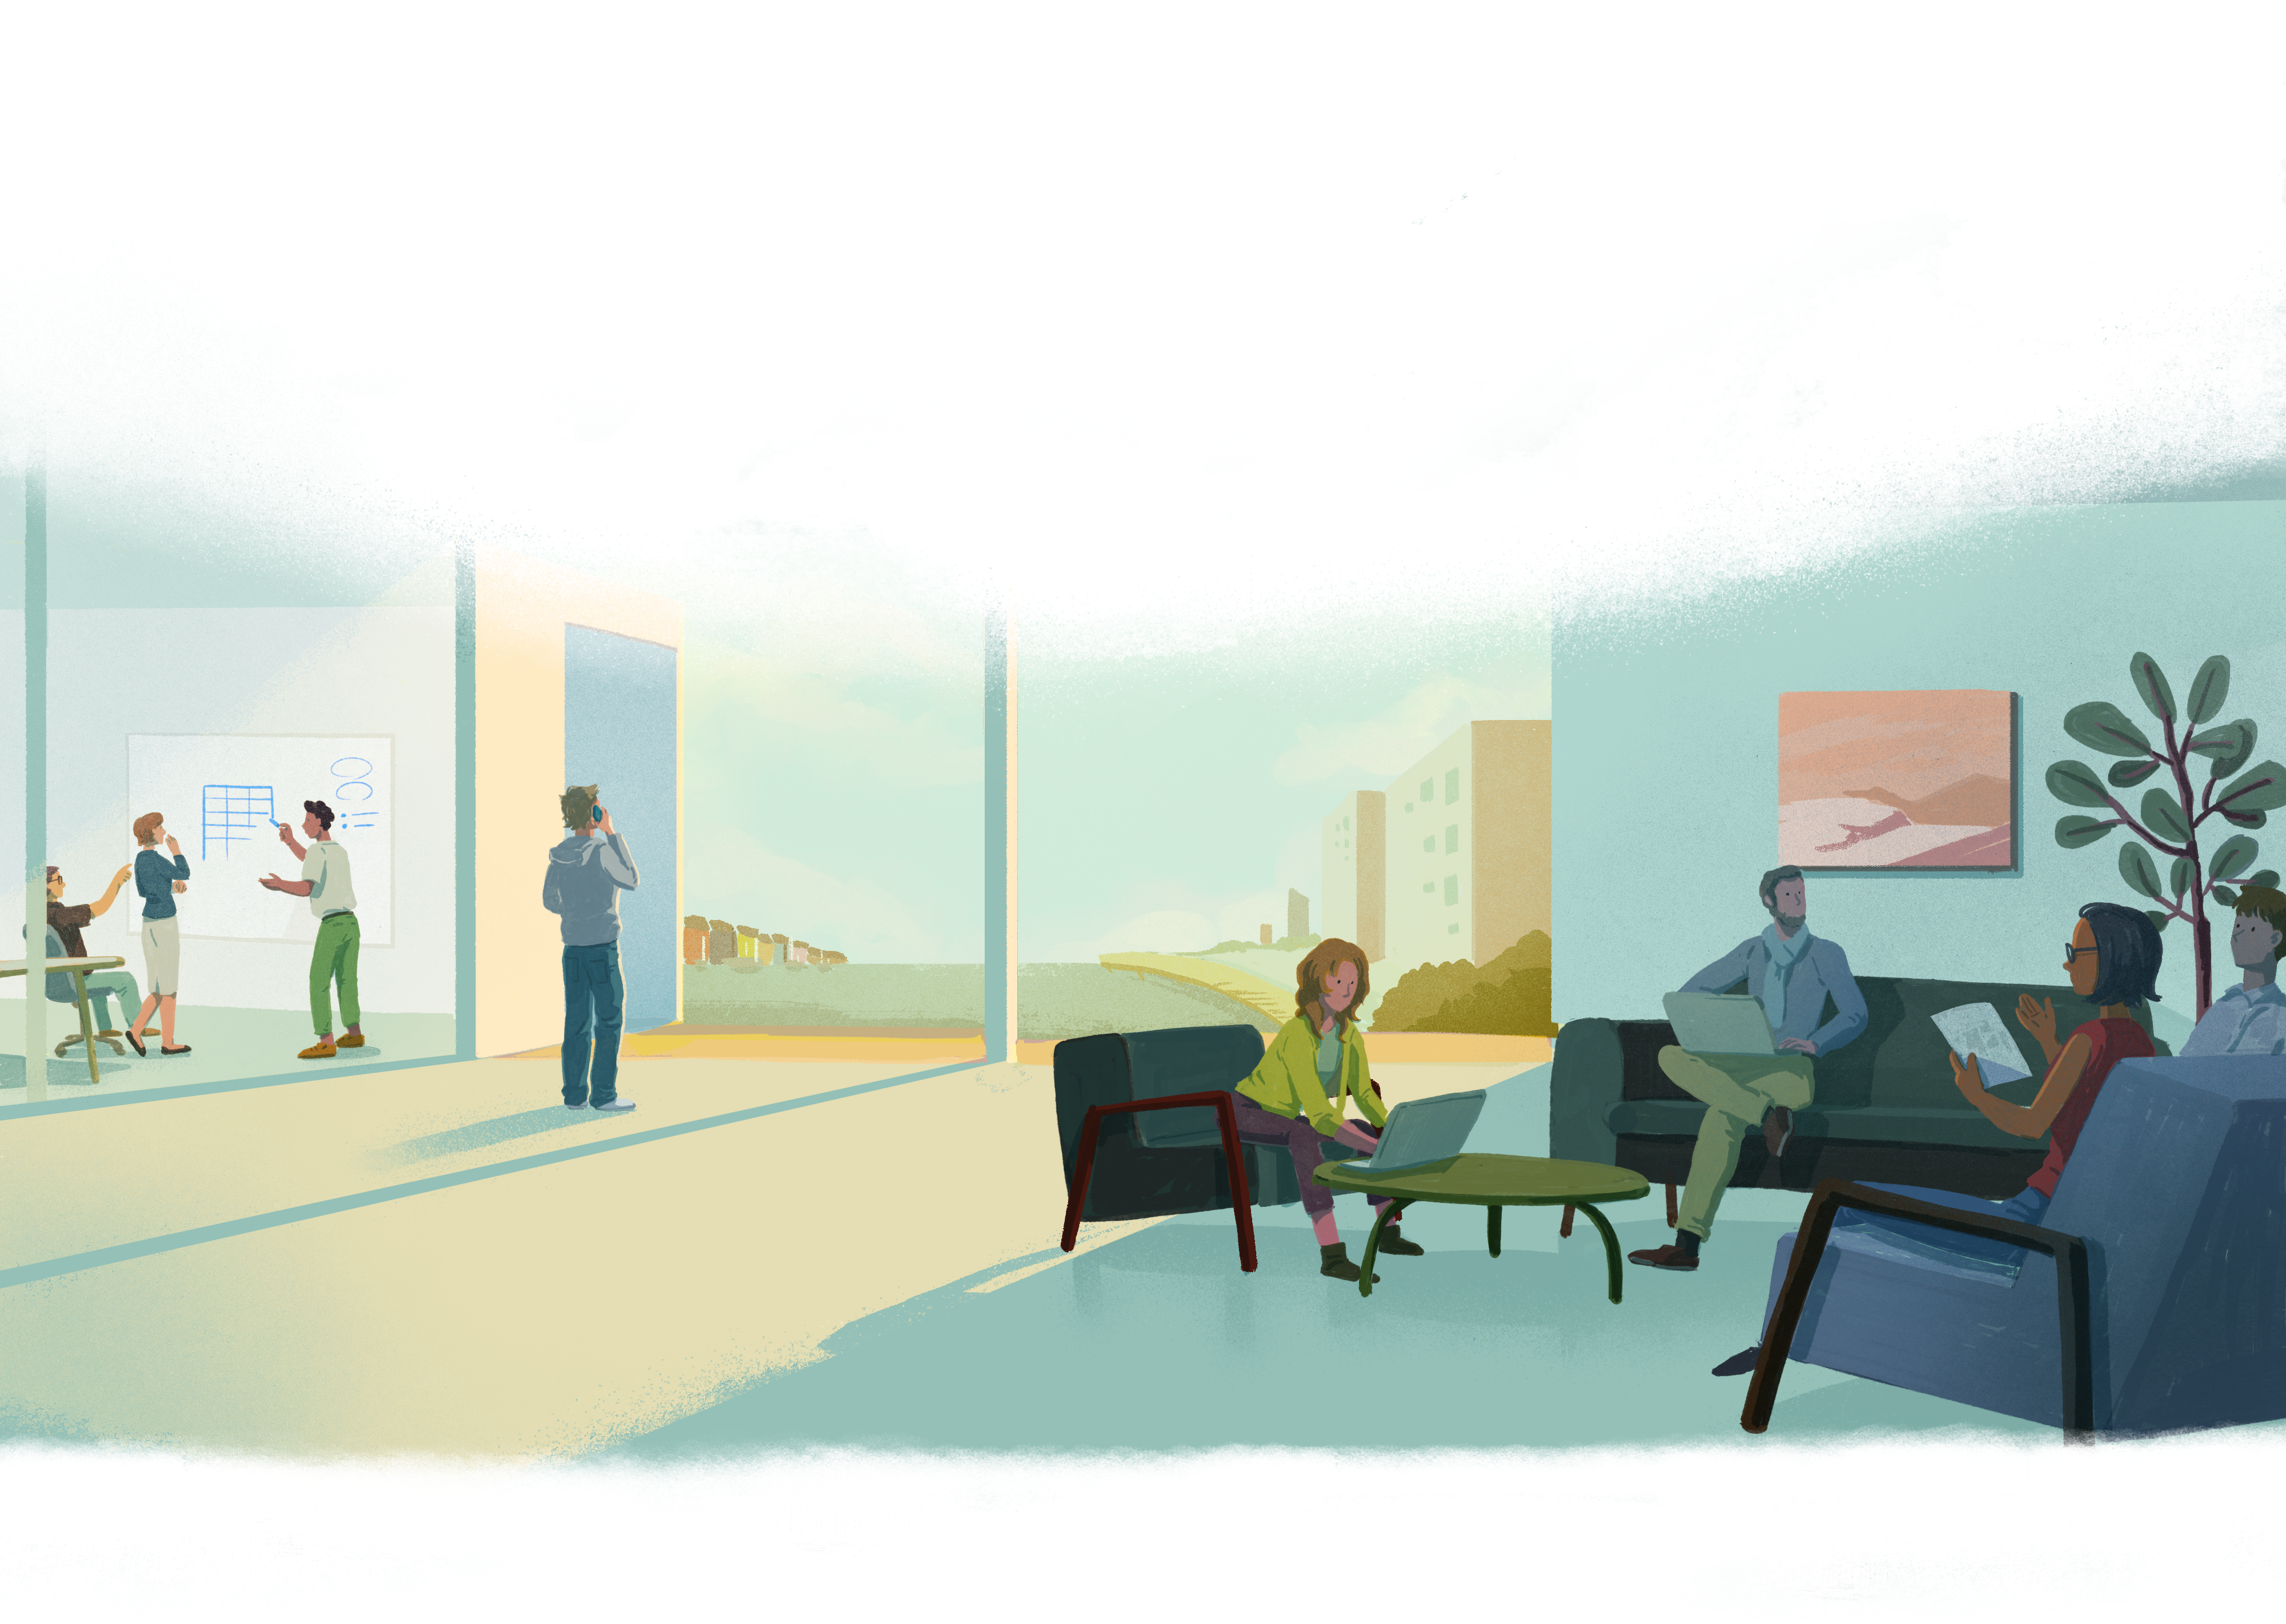
\includegraphics[width=0.95\textwidth]{figures/corti_sketch_office.png}
        \end{column}
    \end{columns}
\end{frame}


\begin{frame}
    \frametitle{Reliability of machine learning systems}
    \begin{itemize}
        \item <1-> \highlight{Data}: Quality, quantity, diversity, bias, privacy, ethics.
        \item <2-> \highlight{Task}: Context, domain, language, culture, purpose.
        \vspace{1em}
        \item <3-> \highlight{Interpretability} of how a model works (transparency, accountability, regulation).
        \item <4-> \highlight{Explainability} of model predictions (trust, understanding, feedback).
        \item <5-> \highlight{Fairness} in treatment of different groups of people.
        \item <6-> \highlight{Robustness} to noise, outliers, distribution shift, and adversarial attacks.
    \end{itemize}
\end{frame}


\tikzstyle{mybox} = [fill, rounded corners, minimum width=140, minimum height=20]
\tikzstyle{myrect} = [fill]

\begin{frame}
    \frametitle{Building a decision-support system}
    \begin{columns}
        \begin{column}{0.6\textwidth}
            Modular approach:
            \begin{itemize}
                \item \highlight{Input}: Speech or text (potentially video, tabular data, images, etc.).
                \item \highlight{Parsing the input}: Representation learning and speech recognition.
                \item \highlight{Output}: Predictions (suggesting, summarizing, classifying, etc.).
            \end{itemize}
        \end{column}
        \begin{column}{0.4\textwidth}
            \resizebox{!}{0.8\textheight}{%
            \begin{tikzpicture}[x=1cm,y=1cm]
                \node<6> [mybox, fill=presentation_orange] at (0,5) (predictions) {};
                \foreach \i in {-11,...,11} {
                    \fill<6>[myrect, fill=presentation_orange_shaded] (0.2*\i,4.8) rectangle ++(0.1,0.4);
                }
                \node<6> [] at (0,5) {\small\textsc{predictions}};
    
                \node<5> [mybox, fill=black!10] at (0,4) (downstream) {\small\textsc{downstream model}};
    
                \node<4> [mybox, fill=presentation_blue] at (0,3) (text) {};
                \foreach \i in {-11,...,11} {
                    \fill<4>[myrect, fill=presentation_blue_shaded] (0.2*\i,2.8) rectangle ++(0.1,0.4);
                }
                \node<4> [] at (0,3) {\small\textsc{text}};
    
                \node<3> [mybox, fill=black!10] at (0,2) (recognition) {\small\textsc{speech recognition}};
    
                \node<2> [mybox, fill=black!10] at (0,1) (representation) {\small\textsc{representation learning}};
    
                \node<1> [mybox, fill=presentation_green] at (0,0) (speech) {};
                \foreach \i in {-11,...,11} {
                    \fill<1>[myrect, fill=presentation_green_shaded] (0.2*\i,-0.2) rectangle ++(0.1,0.4);
                }
                \node<1> [] at (0,0) {\small\textsc{speech}};
    
                \node<7> [draw, rectangle, rounded corners, line width=0.15cm, presentation_red, fit=(speech)(representation)(recognition)(text)(predictions), inner sep=10pt] (uncertainty) {};
                \node<7> [above] at (uncertainty.north) {\small\textsc{uncertainty}};
            \end{tikzpicture}
        }
        \end{column}
    \end{columns}
\end{frame}

% !TEX root = ../presentation.tex
% !BIB program = biber
% !TEX program = xelatex

\hfsetfillcolor{presentation_green}
\hfsetbordercolor{presentation_green}

\newcommand{\tikzoverview}{%
    \resizebox{0.8\textwidth}{!}{%
        \begin{tikzpicture}[x=1cm,y=1cm]
            \node [mybox, fill=presentation_orange] at (0,5) (predictions) {};
            \foreach \i in {-11,...,11} {
                \fill[myrect, fill=presentation_orange_shaded] (0.2*\i,4.8) rectangle ++(0.1,0.4);
            }
            \node [] at (0,5) {\small\textsc{predictions}};

            \node [mybox, fill=black!10] at (0,4) (downstream) {\small\textsc{downstream model}};

            \node [mybox, fill=presentation_blue] at (0,3) (text) {};
            \foreach \i in {-11,...,11} {
                \fill[myrect, fill=presentation_blue_shaded] (0.2*\i,2.8) rectangle ++(0.1,0.4);
            }
            \node [] at (0,3) {\small\textsc{text}};

            \node [mybox, fill=black!10] at (0,2) (recognition) {\small\textsc{speech recognition}};

            \node [mybox, fill=black!10] at (0,1) (representation) {\small\textsc{representation learning}};

            \node [mybox, fill=presentation_green] at (0,0) (speech) {};
            \foreach \i in {-11,...,11} {
                \fill[myrect, fill=presentation_green_shaded] (0.2*\i,-0.2) rectangle ++(0.1,0.4);
            }
            \node [] at (0,0) {\small\textsc{speech}};

            \node [draw, rectangle, rounded corners, line width=0.15cm, presentation_red, fit=(speech)(representation)(recognition)(text)(predictions), inner sep=10pt] (uncertainty) {};
            \node [above] at (uncertainty.north) {\small\textsc{uncertainty}};
        \end{tikzpicture}
    }
}

\newcommand{\tikzhierarchical}{%
    \resizebox{0.8\textwidth}{!}{%
        \begin{tikzpicture}[x=1cm,y=1cm]
            \node [nearly transparent, mybox, fill=presentation_orange] at (0,5) (predictions) {};
            \foreach \i in {-11,...,11} {
                \fill[nearly transparent, myrect, fill=presentation_orange_shaded] (0.2*\i,4.8) rectangle ++(0.1,0.4);
            }
            \node [nearly transparent] at (0,5) {\small\textsc{predictions}};

            \node [nearly transparent, mybox, fill=black!10] at (0,4) (downstream) {\small\textsc{downstream model}};

            \node [nearly transparent, mybox, fill=presentation_blue] at (0,3) (text) {};
            \foreach \i in {-11,...,11} {
                \fill[nearly transparent, myrect, fill=presentation_blue_shaded] (0.2*\i,2.8) rectangle ++(0.1,0.4);
            }
            \node [nearly transparent] at (0,3) {\small\textsc{text}};

            \node [nearly transparent, mybox, fill=black!10] at (0,2) (recognition) {\small\textsc{speech recognition}};

            \node [mybox, fill=black!10] at (0,1) (representation) {\small\textsc{representation learning}};

            \node [nearly transparent, mybox, fill=presentation_green] at (0,0) (speech) {};
            \foreach \i in {-11,...,11} {
                \fill[nearly transparent, myrect, fill=presentation_green_shaded] (0.2*\i,-0.2) rectangle ++(0.1,0.4);
            }
            \node [nearly transparent] at (0,0) {\small\textsc{speech}};

            \node [draw, rectangle, rounded corners, line width=0.15cm, presentation_red, fit=(speech)(representation)(recognition)(text)(predictions), inner sep=10pt] (uncertainty) {};
            \node [above] at (uncertainty.north) {\small\textsc{uncertainty}};
        \end{tikzpicture}
    }
}

\newcommand{\tikzmodelagnostic}{%
    \resizebox{0.8\textwidth}{!}{%
        \begin{tikzpicture}[x=1cm,y=1cm]
            \node [nearly transparent, mybox, fill=presentation_orange] at (0,5) (predictions) {};
            \foreach \i in {-11,...,11} {
                \fill[nearly transparent, myrect, fill=presentation_orange_shaded] (0.2*\i,4.8) rectangle ++(0.1,0.4);
            }
            \node [nearly transparent] at (0,5) {\small\textsc{predictions}};

            \node [nearly transparent, mybox, fill=black!10] at (0,4) (downstream) {\small\textsc{downstream model}};

            \node [nearly transparent, mybox, fill=presentation_blue] at (0,3) (text) {};
            \foreach \i in {-11,...,11} {
                \fill[nearly transparent, myrect, fill=presentation_blue_shaded] (0.2*\i,2.8) rectangle ++(0.1,0.4);
            }
            \node [nearly transparent] at (0,3) {\small\textsc{text}};

            \node [nearly transparent, mybox, fill=black!10] at (0,2) (recognition) {\small\textsc{speech recognition}};

            \node [mybox, fill=black!10] at (0,1) (representation) {\small\textsc{representation learning}};

            \node [nearly transparent, mybox, fill=presentation_green] at (0,0) (speech) {};
            \foreach \i in {-11,...,11} {
                \fill[nearly transparent, myrect, fill=presentation_green_shaded] (0.2*\i,-0.2) rectangle ++(0.1,0.4);
            }
            \node [nearly transparent] at (0,0) {\small\textsc{speech}};

            \node [draw, rectangle, rounded corners, line width=0.15cm, presentation_red, fit=(speech)(representation)(recognition)(text)(predictions), inner sep=10pt] (uncertainty) {};
            \node [above] at (uncertainty.north) {\small\textsc{uncertainty}};
        \end{tikzpicture}
    }
}

\newcommand{\tikzbrief}{%
    \resizebox{0.8\textwidth}{!}{%
        \begin{tikzpicture}[x=1cm,y=1cm]
            \node [nearly transparent, mybox, fill=presentation_orange] at (0,5) (predictions) {};
            \foreach \i in {-11,...,11} {
                \fill[nearly transparent, myrect, fill=presentation_orange_shaded] (0.2*\i,4.8) rectangle ++(0.1,0.4);
            }
            \node [nearly transparent] at (0,5) {\small\textsc{predictions}};

            \node [nearly transparent, mybox, fill=black!10] at (0,4) (downstream) {\small\textsc{downstream model}};

            \node [nearly transparent, mybox, fill=presentation_blue] at (0,3) (text) {};
            \foreach \i in {-11,...,11} {
                \fill[nearly transparent, myrect, fill=presentation_blue_shaded] (0.2*\i,2.8) rectangle ++(0.1,0.4);
            }
            \node [nearly transparent] at (0,3) {\small\textsc{text}};

            \node [nearly transparent, mybox, fill=black!10] at (0,2) (recognition) {\small\textsc{speech recognition}};

            \node [mybox, fill=black!10] at (0,1) (representation) {\small\textsc{representation learning}};

            \node [mybox, fill=presentation_green] at (0,0) (speech) {};
            \foreach \i in {-11,...,11} {
                \fill[myrect, fill=presentation_green_shaded] (0.2*\i,-0.2) rectangle ++(0.1,0.4);
            }
            \node [] at (0,0) {\small\textsc{speech}};

            \node [nearly transparent, draw, rectangle, rounded corners, line width=0.15cm, presentation_red, fit=(speech)(representation)(recognition)(text)(predictions), inner sep=10pt] (uncertainty) {};
            \node [nearly transparent, above] at (uncertainty.north) {\small\textsc{uncertainty}};
        \end{tikzpicture}
    }
}

\newcommand{\tikzbenchmarking}{%
    \resizebox{0.8\textwidth}{!}{%
        \begin{tikzpicture}[x=1cm,y=1cm]
            \node [nearly transparent, mybox, fill=presentation_orange] at (0,5) (predictions) {};
            \foreach \i in {-11,...,11} {
                \fill[nearly transparent, myrect, fill=presentation_orange_shaded] (0.2*\i,4.8) rectangle ++(0.1,0.4);
            }
            \node [nearly transparent] at (0,5) {\small\textsc{predictions}};

            \node [nearly transparent, mybox, fill=black!10] at (0,4) (downstream) {\small\textsc{downstream model}};

            \node [mybox, fill=presentation_blue] at (0,3) (text) {};
            \foreach \i in {-11,...,11} {
                \fill[myrect, fill=presentation_blue_shaded] (0.2*\i,2.8) rectangle ++(0.1,0.4);
            }
            \node [] at (0,3) {\small\textsc{text}};

            \node [mybox, fill=black!10] at (0,2) (recognition) {\small\textsc{speech recognition}};

            \node [mybox, fill=black!10] at (0,1) (representation) {\small\textsc{representation learning}};

            \node [mybox, fill=presentation_green] at (0,0) (speech) {};
            \foreach \i in {-11,...,11} {
                \fill[myrect, fill=presentation_green_shaded] (0.2*\i,-0.2) rectangle ++(0.1,0.4);
            }
            \node [] at (0,0) {\small\textsc{speech}};

            \node [nearly transparent, draw, rectangle, rounded corners, line width=0.15cm, presentation_red, fit=(speech)(representation)(recognition)(text)(predictions), inner sep=10pt] (uncertainty) {};
            \node [nearly transparent, above] at (uncertainty.north) {\small\textsc{uncertainty}};
        \end{tikzpicture}
    }
}

\newcommand{\tikzautomated}{%
    \resizebox{0.8\textwidth}{!}{%
        \begin{tikzpicture}[x=1cm,y=1cm]
            \node [mybox, fill=presentation_orange] at (0,5) (predictions) {};
            \foreach \i in {-11,...,11} {
                \fill[myrect, fill=presentation_orange_shaded] (0.2*\i,4.8) rectangle ++(0.1,0.4);
            }
            \node [] at (0,5) {\small\textsc{predictions}};

            \node [mybox, fill=black!10] at (0,4) (downstream) {\small\textsc{downstream model}};

            \node [mybox, fill=presentation_blue] at (0,3) (text) {};
            \foreach \i in {-11,...,11} {
                \fill[myrect, fill=presentation_blue_shaded] (0.2*\i,2.8) rectangle ++(0.1,0.4);
            }
            \node [] at (0,3) {\small\textsc{text}};

            \node [nearly transparent, mybox, fill=black!10] at (0,2) (recognition) {\small\textsc{speech recognition}};

            \node [nearly transparent, mybox, fill=black!10] at (0,1) (representation) {\small\textsc{representation learning}};

            \node [nearly transparent, mybox, fill=presentation_green] at (0,0) (speech) {};
            \foreach \i in {-11,...,11} {
                \fill[nearly transparent, myrect, fill=presentation_green_shaded] (0.2*\i,-0.2) rectangle ++(0.1,0.4);
            }
            \node [nearly transparent] at (0,0) {\small\textsc{speech}};

            \node [nearly transparent, draw, rectangle, rounded corners, line width=0.15cm, presentation_red, fit=(speech)(representation)(recognition)(text)(predictions), inner sep=10pt] (uncertainty) {};
            \node [nearly transparent, above] at (uncertainty.north) {\small\textsc{uncertainty}};
        \end{tikzpicture}
    }
}

\newcommand{\tikzretrospective}{%
    \resizebox{0.8\textwidth}{!}{%
        \begin{tikzpicture}[x=1cm,y=1cm]
            \node [mybox, fill=presentation_orange] at (0,5) (predictions) {};
            \foreach \i in {-11,...,11} {
                \fill[myrect, fill=presentation_orange_shaded] (0.2*\i,4.8) rectangle ++(0.1,0.4);
            }
            \node [] at (0,5) {\small\textsc{predictions}};

            \node [mybox, fill=black!10] at (0,4) (downstream) {\small\textsc{downstream model}};

            \node [mybox, fill=presentation_blue] at (0,3) (text) {};
            \foreach \i in {-11,...,11} {
                \fill[myrect, fill=presentation_blue_shaded] (0.2*\i,2.8) rectangle ++(0.1,0.4);
            }
            \node [] at (0,3) {\small\textsc{text}};

            \node [mybox, fill=black!10] at (0,2) (recognition) {\small\textsc{speech recognition}};

            \node [mybox, fill=black!10] at (0,1) (representation) {\small\textsc{representation learning}};

            \node [mybox, fill=presentation_green] at (0,0) (speech) {};
            \foreach \i in {-11,...,11} {
                \fill[myrect, fill=presentation_green_shaded] (0.2*\i,-0.2) rectangle ++(0.1,0.4);
            }
            \node [] at (0,0) {\small\textsc{speech}};

            \node [draw, rectangle, rounded corners, line width=0.15cm, presentation_red, fit=(speech)(representation)(recognition)(text)(predictions), inner sep=10pt] (uncertainty) {};
            \node [above] at (uncertainty.north) {\small\textsc{uncertainty}};
        \end{tikzpicture}
    }
}

\section{Overview}

% Go through the papers of the thesis while showing the graphic of their themes.
\begin{frame}
    \frametitle{Thesis}
    \begin{columns}
        \begin{column}{0.6\textwidth}
            \begin{table}
                \resizebox{\textwidth}{!}{%
                \begin{tabular}{l l l l}
                    & {\color<2->{black!20}   \makecell[l]{\textsc{\itshape chapter 1-3}}} & {\color<2->{black!20}    \bfseries \scshape \Large \makecell[l]{introduction, research questions, and background}} & \\
                    \addlinespace[0.5em]
                    \midrule
                    \addlinespace[0.5em]
                    
                    \tikzmarkin<2>{hierarchical-1}(0.1,-0.3)(-0.1,0.4)
                    & {\color<2->{black}\makecell[l]{\textsc{\itshape chapter 4}}}         & {\color<2->{black} \bfseries \scshape \Large \makecell[l]{hierarchical vaes know what they don't know}} & \tikzmarkend{hierarchical-1} \\
                    \addlinespace[0.5em]
                    \addlinespace[0.5em]

                    \tikzmarkin<2>{modelagnostic-1}(0.1,-0.4)(-0.1,0.6)
                    & {\color<2->{black}\makecell[l]{\textsc{\itshape chapter 5}\\\\}}     & {\color<2->{black} \bfseries \scshape \Large \makecell[l]{model-agnostic out-of-distribution detection\\ using combined statistical tests}} & \tikzmarkend{modelagnostic-1} \\
                    \addlinespace[0.5em]
                    \addlinespace[0.5em]

                    \tikzmarkin<3>{brief-1}(0.1,-0.4)(-0.1,0.6)
                    & {\color<2->{black}\makecell[l]{ \textsc{\itshape chapter 6}\\\\}}    & {\color<2->{black} \bfseries \scshape \Large \makecell[l]{a brief overview of unsupervised speech \\representation learning}} & \tikzmarkend{brief-1} \\
                    \addlinespace[0.5em]
                    \addlinespace[0.5em]

                    \tikzmarkin<4>{benchmarking-1}(0.1,-0.3)(-0.1,0.4)
                    & {\color<2->{black}\makecell[l]{\textsc{\itshape chapter 7}}}         & {\color<2->{black} \bfseries \scshape \Large \makecell[l]{benchmarking latent variable models for speech}} & \tikzmarkend{benchmarking-1} \\
                    \addlinespace[0.5em]
                    \addlinespace[0.5em]

                    \tikzmarkin<5>{automated-1}(0.1,-0.4)(-0.1,0.6)
                    & {\color<2->{black}\makecell[l]{\textsc{\itshape chapter 8}\\\\}}     & {\color<2->{black} \bfseries \scshape \Large \makecell[l]{automated medical coding on mimic-iii and \\mimic-iv: a critical review and replicability study}} & \tikzmarkend{automated-1} \\
                    \addlinespace[0.5em]
                    \addlinespace[0.5em]

                    \tikzmarkin<6>{retrospective-1}(0.1,-0.4)(-0.1,0.6)
                    & {\color<2->{black}\makecell[l]{\textsc{\itshape chapter 9}\\\\}}     & {\color<2->{black} \bfseries \scshape \Large \makecell[l]{a retrospective study on machine learning-\\assisted stroke recognition for medical helpline calls}} & \tikzmarkend{retrospective-1} \\
                    \addlinespace[0.5em]
                    \midrule
                    \addlinespace[0.5em]

                    & {\color<2->{black!20}\makecell[l]{\textsc{\itshape chapter 10}}}        & {\color<2->{black!20} \bfseries \scshape \Large \makecell[l]{discussion and conclusion}} & \\
                \end{tabular}
                }
            \end{table}
        \end{column}
        \begin{column}{0.4\textwidth}
            \begin{figure}
                \centering
                \begin{overprint}
                    \onslide<1>\tikzoverview
                    \onslide<2>\tikzhierarchical
                    % \onslide<2>\tikzmodelagnostic
                    \onslide<3>\tikzbrief
                    \onslide<4>\tikzbenchmarking
                    \onslide<5>\tikzautomated
                    \onslide<6>\tikzretrospective
                \end{overprint}
            \end{figure}
        \end{column}
    \end{columns}

    \note[item]<1->{So how does the thesis tackle this problem of building such a system?}
    \note[item]<2->{First we examine how a certain class of generative models can be used to detect data that is different from training data.}
    \note[item]<2->{In our second paper we generalize this to be model-agnostic and phrased as a statistical test.}
    \note[item]<3->{We then take a step back and provide an overview of modern methods for unsupervised speech representation learning.}
    \note[item]<4->{We then benchmark some of these methods, generative latent variable models, on likelihood and automatic speech recognition.}
    \note[item]<5->{We then move to a different domain, medical coding, and provide a critical review of recent works.}
    \note[item]<6->{Finally, we provide a retrospective study on a machine learning-assisted stroke recognition system for medical helpline calls.}
    \end{frame}


\hfsetfillcolor{white}
\hfsetbordercolor{white}


% Grey out scoped-out papers in the overview
\begin{frame}
    \frametitle{Presentation}
    \begin{columns}
        \begin{column}{0.6\textwidth}
            \begin{table}
                \resizebox{\textwidth}{!}{%
                \begin{tabular}{l l l l}
                    & {\color<2->{black}   \makecell[l]{\textsc{\itshape chapter 1-3}}} & {\color<2->{black}    \bfseries \scshape \Large \makecell[l]{introduction, research questions, and background}} & \\
                    \addlinespace[0.5em]
                    \midrule
                    \addlinespace[0.5em]
                    
                    \tikzmarkin<1->{hierarchical-2}(0.1,-0.3)(-0.1,0.4)
                    & {\color<2->{black}\makecell[l]{\textsc{\itshape chapter 4}}}         & {\color<2->{black} \bfseries \scshape \Large \makecell[l]{hierarchical vaes know what they don't know}} & \tikzmarkend{hierarchical-2} \\
                    \addlinespace[0.5em]
                    \addlinespace[0.5em]

                    \tikzmarkin<1->{modelagnostic-2}(0.1,-0.4)(-0.1,0.6)
                    & {\color<2->{dtured!40}\makecell[l]{\textsc{\itshape chapter 5}\\\\}}     & {\color<2->{dtured!40} \bfseries \scshape \Large \makecell[l]{model-agnostic out-of-distribution detection\\ using combined statistical tests}} & \tikzmarkend{modelagnostic-2} \\
                    \addlinespace[0.5em]
                    \addlinespace[0.5em]

                    \tikzmarkin<1->{brief-2}(0.1,-0.4)(-0.1,0.6)
                    & {\color<2->{black}\makecell[l]{ \textsc{\itshape chapter 6}\\\\}}    & {\color<2->{black} \bfseries \scshape \Large \makecell[l]{a brief overview of unsupervised speech \\representation learning}} & \tikzmarkend{brief-2} \\
                    \addlinespace[0.5em]
                    \addlinespace[0.5em]

                    \tikzmarkin<1->{benchmarking-2}(0.1,-0.3)(-0.1,0.4)
                    & {\color<2->{dtured!40}\makecell[l]{\textsc{\itshape chapter 7}}}         & {\color<2->{dtured!40} \bfseries \scshape \Large \makecell[l]{benchmarking latent variable models for speech}} & \tikzmarkend{benchmarking-2} \\
                    \addlinespace[0.5em]
                    \addlinespace[0.5em]

                    \tikzmarkin<1->{automated-2}(0.1,-0.4)(-0.1,0.6)
                    & {\color<2->{dtured!40}\makecell[l]{\textsc{\itshape chapter 8}\\\\}}     & {\color<2->{dtured!40} \bfseries \scshape \Large \makecell[l]{automated medical coding on mimic-iii and \\mimic-iv: a critical review and replicability study}} & \tikzmarkend{automated-2} \\
                    \addlinespace[0.5em]
                    \addlinespace[0.5em]

                    \tikzmarkin<1->{retrospective-2}(0.1,-0.4)(-0.1,0.6)
                    & {\color<2->{black}\makecell[l]{\textsc{\itshape chapter 9}\\\\}}     & {\color<2->{black} \bfseries \scshape \Large \makecell[l]{a retrospective study on machine learning-\\assisted stroke recognition for medical helpline calls}} & \tikzmarkend{retrospective-2} \\
                    \addlinespace[0.5em]
                    \midrule
                    \addlinespace[0.5em]

                    & {\color<2->{black!20}\makecell[l]{\textsc{\itshape chapter 10}}}        & {\color<2->{black!20} \bfseries \scshape \Large \makecell[l]{discussion and conclusion}} & \\
                \end{tabular}
                }
            \end{table}
        \end{column}
        \begin{column}{0.4\textwidth}
            \tikzstyle{mybox} = [fill, rounded corners, minimum width=140, minimum height=20]
            \tikzstyle{myrect} = [fill]
            \begin{figure}
                \centering
                \begin{overprint}
                    \onslide<1->\tikzoverview
                \end{overprint}
            \end{figure}
        \end{column}
    \end{columns}
\end{frame}


% % \part{Unsupervised Out-of-Distribution Detection}
% % !TEX root = ../presentation.tex
% !BIB program = biber
% !TEX program = xelatex

\section*{overview}

\begin{frame}
    \frametitle{Presentation}
    \begin{columns}
        \begin{column}{0.6\textwidth}
            \begin{table}
                \resizebox{\textwidth}{!}{%
                \begin{tabular}{l l l l}
                    & {\color<2->{black!20}   \makecell[l]{\textsc{\itshape chapter 1-3}}} & {\color<2->{black!20}    \bfseries \scshape \Large \makecell[l]{introduction, research questions, and background}} & \\
                    \addlinespace[0.5em]
                    \midrule
                    \addlinespace[0.5em]

                    \tikzmarkin<1->{hierarchical-3}(0.1,-0.3)(-0.1,0.4)
                    & {\color<2->{black}\makecell[l]{\textsc{\itshape chapter 4}}}         & {\color<2->{black} \bfseries \scshape \Large \makecell[l]{hierarchical vaes know what they don't know}} & \tikzmarkend{hierarchical-3} \\
                    \addlinespace[0.5em]
                    \addlinespace[0.5em]

                    % \tikzmarkin<1->{modelagnostic-3}(0.1,-0.4)(-0.1,0.6)
                    % & {\color<2->{black!20}\makecell[l]{\textsc{\itshape chapter 5}\\\\}}     & {\color<2->{black!20} \bfseries \scshape \Large \makecell[l]{model-agnostic out-of-distribution detection\\ using combined statistical tests}} & \tikzmarkend{modelagnostic-3} \\
                    % \addlinespace[0.5em]
                    % \addlinespace[0.5em]

                    \tikzmarkin<1->{brief-3}(0.1,-0.4)(-0.1,0.6)
                    & {\color<2->{black!20}\makecell[l]{ \textsc{\itshape chapter 6}\\\\}}    & {\color<2->{black!20} \bfseries \scshape \Large \makecell[l]{a brief overview of unsupervised speech \\representation learning}} & \tikzmarkend{brief-3} \\
                    \addlinespace[0.5em]
                    \addlinespace[0.5em]

                    % \tikzmarkin<1->{benchmarking-3}(0.1,-0.3)(-0.1,0.4)
                    % & {\color<2->{black!20}\makecell[l]{\textsc{\itshape chapter 7}}}         & {\color<2->{black!20} \bfseries \scshape \Large \makecell[l]{benchmarking latent variable models for speech}} & \tikzmarkend{benchmarking-3} \\
                    % \addlinespace[0.5em]
                    % \addlinespace[0.5em]

                    % \tikzmarkin<1->{automated-3}(0.1,-0.4)(-0.1,0.6)
                    % & {\color<2->{black!20}\makecell[l]{\textsc{\itshape chapter 8}\\\\}}     & {\color<2->{black!20} \bfseries \scshape \Large \makecell[l]{automated medical coding on mimic-iii and \\mimic-iv: a critical review and replicability study}} & \tikzmarkend{automated-3} \\
                    % \addlinespace[0.5em]
                    % \addlinespace[0.5em]

                    \tikzmarkin<1->{retrospective-3}(0.1,-0.4)(-0.1,0.6)
                    & {\color<2->{black!20}\makecell[l]{\textsc{\itshape chapter 9}\\\\}}     & {\color<2->{black!20} \bfseries \scshape \Large \makecell[l]{a retrospective study on machine learning-\\assisted stroke recognition for medical helpline calls}} & \tikzmarkend{retrospective-3} \\
                    \addlinespace[0.5em]
                    \midrule
                    \addlinespace[0.5em]

                    & {\color<2->{black!20}\makecell[l]{\textsc{\itshape chapter 10}}}        & {\color<2->{black!20} \bfseries \scshape \Large \makecell[l]{discussion and conclusion}} & \\
                \end{tabular}
                }
            \end{table}
        \end{column}
        \begin{column}{0.4\textwidth}
            \tikzstyle{mybox} = [fill, rounded corners, minimum width=140, minimum height=20]
            \tikzstyle{myrect} = [fill]
            \begin{figure}
                \centering
                \begin{overprint}
                    \onslide<1>\tikzoverview
                    \onslide<2>\tikzhierarchical
                \end{overprint}
            \end{figure}
        \end{column}
    \end{columns}
\end{frame}


% % !TEX root = ../presentation.tex
% !BIB program = biber
% !TEX program = xelatex

\section{hierarchical vaes know what they don't know}


\frame{
    \frametitle{Defining OOD detection}
    \begin{columns}
        \begin{column}{0.5\textwidth}
            Enable models to distinguish the training data distribution $p(\xb)$ from any other distribution $\tilde{p}(\xb)$.
            \vspace{3mm}
            Do this for any given single observation, i.e. answer the question:
            \vspace{3mm}
            \begin{center}
                "Was $\xb$ sampled from $p(\xb)$ or not?"
            \end{center}
        \end{column}
        \begin{column}{0.5\textwidth}
            \begin{figure}[\textwidth]
                \centering
                \begin{tikzpicture}
                        \begin{axis}[
                            name=axistop,
                            domain=0:13,samples=100,
                            height=4.5cm, width=8cm,
                            xtick=\empty,
                            every axis plot/.append style={very thick,smooth}
                        ]
                            \addplot [name path=p1, color=red!50!black] {gauss(5,1)};
                            \addplot [name path=p2, color=black] {gauss(8,1)};
                            \path[name path=axis] (axis cs:0,0) -- (axis cs:10,0);
                            \addlegendentry{$p(\xb)$}
                            \addlegendentry{$\tilde{p}(\xb)$}
                        \end{axis}
                        \path (axistop.south) ++ (0,-0.4cm) coordinate (test);
                        \begin{axis}[
                            name=axisbottom,
                            anchor=north,
                            shift=(test),
                            domain=0:13,samples=100,
                            height=4.5cm, width=8cm,
                            every axis plot/.append style={very thick,smooth}
                        ]
                            \addplot [name path=p1, color=red!50!black] {gauss(4,0.5)};
                            \addplot [name path=p2, color=black] {gauss(9,0.5)};
                            \path[name path=axis] (axis cs:0,0) -- (axis cs:10,0);
                            \addlegendentry{$p(\xb)$}
                            \addlegendentry{$\tilde{p}(\xb)$}
                        \end{axis}
                \end{tikzpicture}
            \end{figure}
        \end{column}
    \end{columns}
}


\frame{
    \frametitle{In distribution?}
    \begin{figure}[\textwidth]
        \centering
        \includegraphics[scale=0.6]{figures/dataexamples_shuffled.pdf}
    \end{figure}
}


\frame{
    \frametitle{Out of distribution?}
    \begin{figure}[\textwidth]
        \centering
        \includegraphics[scale=0.6]{figures/dataexamples.pdf}
    \end{figure}
}


\frame{
    \frametitle{Problem and Contributions}
    \begin{itemize}
        \item Deep generative models often fail at OOD detection task when using their likelihood estimate as the score function \cite{nalisnick_deep_2019} by, perhaps surprisingly, assigning \highlight{higher likelihoods to OOD data}.
        \item Contributions:
        \begin{itemize}
            \item We provide evidence that out-of-distribution detection fails due to learned low-level features that generalize across datasets.
            \item We present a new score for OOD detection with hierarchical VAEs that alleviates this issue.
        \end{itemize}  
    \end{itemize}
}


% \section{Latent variable models}

\begin{frame}{Hierarchical VAE}
  \begin{columns}
      \begin{column}{0.7\textwidth}
          We choose the hierarchical VAE as our model \cite{kingma_autoencoding_2014, rezende_stochastic_2014}.
          \begin{equation*}
              p_\theta(\xb) = \int p_\theta(\xb,\zb) \text{d}\zb = \int p_\theta(\xb|\zb)p_\theta(\zb) \text{d}\zb
          \end{equation*}
          Specifically we use
          
          \begin{enumerate}
              \item a three-layered hierarchical VAE with bottom-up inference and deterministic skip-connections for both inference and generation.
              \begin{align*}
                  \text{Generative model: }\quad p_\theta(\xb|\zb) &= p_\theta(\xb|\zb_1) p_\theta(\zb_1|\zb_2) p(\zb_3),\\
                  \text{Inference model: }\quad q_\phi(\zb|\xb) &= q_\phi(\zb_1|\xb)q_\phi(\zb_2|\zb_1)q_\phi(\zb_3|\zb_2).
              \end{align*}
              \item a ten-layered layered Bidirectional-Inference Variational Autoencoder (BIVA) \cite{maaloe_biva_2019}.
          \end{enumerate} 
      \end{column}
      \begin{column}{0.3\textwidth}
          \begin{figure}[.5\textwidth]
          \tikz{
          % inference
          % nodes
          \node[obs] (x_inf) {$\xb$};%
          \node[latent,above=.75cm of x_inf](z1_inf){$\zb_1$}; %
          \node[latent,above=.75cm of z1_inf](z2_inf){$\zb_2$}; %
          \node[latent,above=.75cm of z2_inf](z3_inf){$\zb_3$}; %
          \node[above=of z3_inf, yshift=-1.cm] (phi) {$q_\phi(\zb|\xb)$}; 
          
          % edges
          \edge[]{x_inf}{z1_inf};
          \edge[]{z1_inf}{z2_inf};
          \edge[]{z2_inf}{z3_inf};
          \edge[dashed, bend left]{x_inf}{z2_inf};
          \edge[dashed, bend left]{x_inf}{z3_inf};
          
          % generative
          % nodes$
          \node[obs,right=0.75cm of x_inf] (x_gen) {$\xb$};%
          \node[latent,above=.75cm of x_gen](z1_gen){$\zb_1$}; %
          \node[latent,above=.75cm of z1_gen](z2_gen){$\zb_2$}; %
          \node[latent,above=.75cm of z2_gen](z3_gen){$\zb_3$}; %
          \node[above=of z3_gen, yshift=-1.cm] (theta) {$p_\theta(\xb,\zb)$}; 
          
          % edges
          \edge[]{z3_gen}{z2_gen};
          \edge[]{z2_gen}{z1_gen};
          \edge[]{z1_gen}{x_gen};
          \edge[dashed, bend left]{z2_gen}{x_gen};
          \edge[dashed, bend left]{z3_gen}{x_gen};
          }
          \end{figure}
      \end{column}
  \end{columns}
\end{frame}


\begin{frame}
    \frametitle{Out-of-distribution detection with hierarchical VAEs}
    \begin{columns}[t]
        \begin{column}{0.4\textwidth}
            \begin{itemize}
                \item Generative models learn to approximate the \textbf{data distribution} $p(\xb)$.
                \item The likelihood of the model given a sample $\xb$ is a measure of how well the model \textbf{explains the data}.
                \item \textbf{Model likelihood} has long been thought of as useful for OOD detection \cite{bishop_novelty_1994}.
            \end{itemize}
        \end{column}
        \begin{column}{0.6\textwidth}
            \begin{overprint}
                \onslide<2>
                \begin{figure}
                    \centering
                    \includegraphics[width=\textwidth]{../graphics/paper_hierarchical/densities-FashionMNIST-test-MNIST-test-bpp-k-0_sohau.pdf}
                \end{figure}
            \end{overprint}
        \end{column}
    \end{columns}
\end{frame}


% \section{Identifying the issue}


\frame{
    \frametitle{What is wrong with the ELBO for OOD detection?}
    We can split the ELBO into two terms
    \begin{equation}
        \mathcal{L}(\xb;\theta,\phi) 
        = \mathbb{E}_{q_\phi(\zb|\xb)} \left[ \log \frac{p_\theta(\xb,\zb)}{q_\phi(\zb|\xb)} \right] 
        = \underbrace{\mathbb{E}_{q_\phi(\zb|\xb)}[\log p_\theta(\xb|\zb)]}_{\text{reconstruction likelihood}} - \underbrace{D_{\mathrm{KL}}( q_\phi(\zb|\xb) || p(\zb))}_{\text{regularization penalty}} \ .
    \end{equation}
    The first term is high if the data is well-explained by $\zb$.

    \vspace{3mm}
    The second term we can rewrite as,
    \begin{equation}
        D_{\mathrm{KL}}( q_\phi(\zb|\xb) || p(\zb)) = \mathbb{E}_{q_\phi(\zb|\xb)} \Big[ \textstyle\sum_{i=1}^{L-1} \log \frac{p_\theta(\zb_i|\zb_{i+1})}{q_\phi(\zb_i|\zb_{i-1})} + \log \frac{p_\theta(\zb_L)}{q_\phi(\zb_L|\zb_{L-1})} \Big] \ .
    \end{equation}
    The absolute log-ratios grow with $\mathrm{dim}(\zb_i)$ since the log probability terms are computed by summing over the dimensionality of $\zb_i$.
    
    \vspace{3mm}
}


\frame{
    \frametitle{What do the lowest latent variables code for?}
    
    Absolute Pearson correlations between data representations in all layers of the inference network of a hierarchical VAE trained on FashionMNIST and of another trained on MNIST. 
    \vspace{0.3cm}

    Correlation computed between the representations of the two different models given the same data, FashionMNIST (top) and MNIST (bottom).
    
    \begin{figure}[\textwidth]
        \centering
        \includegraphics[scale=0.75]{../graphics/paper_hierarchical/feature-correlation-heatmap2.pdf}
        % \caption{Caption}
        % \label{fig:my_label}
    \end{figure}
}


\section{The $\mathcal{L}^{>k}$ likelihood bound}


\frame{
    \frametitle{An alternative likelihood bound, $\mathcal{L}^{>k}$}
    An alternative version of the ELBO that only partially uses the approximate posterior can be written as \cite{maaloe_biva_2019}
    \begin{equation}
        \mathcal{L}^{>k}(\xb; \theta, \phi) = \mathbb{E}_{p_\theta(\zb_{\leq k}|\zb{>k})q_\phi(\zb_{>k}|\xb)} \left[ \log \frac{p_\theta(\xb|\zb)p_\theta(\zb_{>k})}{q_\phi(\zb_{>k}|\xb)} \right]
    \end{equation}
    
    Here, we have replaced the approximate posterior $q_\phi(\zb|\xb)$ with a different proposal distribution that combines part of the approximate posterior with the conditional prior, namely
    
    $$p_\theta(\zb_{\leq k}|\zb_{>k})q_\phi(\zb_{>k}|\xb)$$
    
    This bound uses the conditional prior for the lowest latent variables in the hierarchy.
}


\section{Likelihood ratio}


\frame{
    \frametitle{Likelihood ratios}
    We can use our new bound to compute the score used in a standard likelihood ratio test \cite{buse_likelihood_1982}.
    \begin{equation}\label{eq:llr-as-difference-in-likelihoods}
        LLR^{>k}(\xb) \equiv \mathcal{L}(\xb) - \mathcal{L}^{>k}(\xb) \ .
    \end{equation}
    We can inspect what this likelihood-ratio measures by considering the exact form of our bounds.
    \begin{align}
        \mathcal{L}      &= \log p_\theta(\xb) - D_{\mathrm{KL}}\left( q_\phi(\zb|\xb) || p_\theta(\zb|\xb)\right), \label{eq:likelihoods-as-exact} \\ 
        \mathcal{L}^{>k} &= \log p_\theta(\xb) - D_{\mathrm{KL}}\left( p_\theta(\zb_{\leq }|\zb_{>k}) q_\phi(\zb_{>k}|\xb) || p_\theta(\zb|\xb)\right) \notag \ .
    \end{align}
    In the likelihood ratio the reconstruction terms cancel out and only the KL-divergences from the approximate to the true posterior remain.
    \begin{align}\label{eq:llr-as-kls}
        LLR^{>k}(\xb) &= - D_{\mathrm{KL}}\left( q_\phi(\zb|\xb) || p_\theta(\zb|\xb)\right) \\
                     &\quad + D_{\mathrm{KL}}\left( p_\theta(\zb_{\leq }|\zb_{>k}) q_\phi(\zb_{>k}|\xb) || p_\theta(\zb|\xb)\right) \ . \notag
    \end{align}
}


\frame{
    \frametitle{Importance sampling the ELBO}
    The importance weighted autoencoder (IWAE) bound is tight with the true likelihood in the limit of infinite samples, $S\rightarrow\infty$ \cite{burda_importance_2016},
    \begin{equation}\label{eq:iw-bound}
        \mathcal{L}_{S} = \mathbb{E}_{q(\zb|\xb)}\left[ \log \frac{1}{N} \sum_{s=1}^{S} \frac{p(\xb, \zb^{(s)})}{q(\zb^{(s)}|\xb)} \right] \leq \log p_\theta(\xb) \ ,
    \end{equation}

    \vspace{3mm}

    Consequently, by importance sampling the ELBO, the associated KL-divergence vanishes and our likelihood ratio reduces to the KL-divergence of $\mathcal{L}^{>k}$.

    \begin{equation}\label{eq:llr-as-kls-iwae-reduced}
        LLR^{>k}_{S}(\xb) \rightarrow D_{\mathrm{KL}}( p(\zb_{\leq }|\zb_{>k}) q(\zb_{>k}|\xb) || p(\zb|\xb)) \ .
    \end{equation}

    $LLR^{>k}_{S}(\xb)$ performs KL-divergence-based OOD detection using top-most latent variables.
}


\frame{
    \frametitle{Results with $LLR^{>k}$}
    \begin{figure}[\textwidth]
    \centering
    \begin{subfigure}[c]{0.49\textwidth}
        \centering
        \includegraphics[width=\textwidth]{../graphics/paper_hierarchical/roc-FashionMNIST-test-MNIST-test-ll-and-llr-IW250_sohau.pdf}
        \caption{FashionMNIST HVAE evaluated on MNIST}
    \end{subfigure}
    \hfill
    \begin{subfigure}[c]{0.49\textwidth}
        \centering
        \includegraphics[width=\textwidth]{../graphics/paper_hierarchical/roc-biva-CIFAR10-SVHN-ll-and-llr_sohau.pdf}
        \caption{CIFAR10 BIVA evaluated on SVHN}
    \end{subfigure}
    \end{figure}
}


\begin{frame}
    \frametitle{Selecting the value of $k$}
    \begin{itemize}
        \item Use validation OOD dataset(s).
        \item Compute $LLR^{>k}$ for different values of $k$ and select the one that maximizes the AUROC.
        \item Compute feature correlations for different values of $k$ and select $k$ at the drop.
    \end{itemize}
    \begin{figure}
        \centering
        \includegraphics[width=0.9\textwidth]{../graphics/paper_hierarchical/feature-correlation-heatmap2.pdf}
    \end{figure}
\end{frame}


\begin{frame}
    \frametitle{Results on FashionMNIST/MNIST}
    \begin{table}
        \centering
        \resizebox*{!}{0.87\textheight}{%
        \begin{tabular}{lrrr}
            \toprule
            Method & AUROC$\uparrow$ & AUPRC$\uparrow$ & FPR80$\downarrow$ \\
            \midrule
            \multicolumn{4}{c}{\textbf{FashionMNIST (in) / MNIST (out)}} \\
            \midrule
            \multicolumn{4}{l}{\textbf{Use prior knowledge of OOD}} \\
            Backgr. contrast. LR (PixelCNN) {\parencite{ren_likelihood_2019}}               & $0.994$ & $0.993$ & $0.001$ \\
            Backgr. contrast. LR (VAE) {\parencite{choi_waic_2019}}                    & $0.924$ & - & - \\
            Binary classifier {\parencite{ren_likelihood_2019}}                              & $0.455$ & $0.505$ & $0.886$ \\ % 6
            $p(\hat{y} | \xb)$ with OOD as noise class {\parencite{ren_likelihood_2019}}     & $0.877$ & $0.871$ & $0.195$ \\ % 7
            $p(\hat{y} | \xb)$ with calibration on OOD {\parencite{ren_likelihood_2019}}     & $0.904$ & $0.895$ & $0.139$ \\ % 8
            Input complexity ($S$, Glow) \parencite{hendrycks_deep_2019}                    & $0.998$ & - & - \\
            Input complexity ($S$, PixelCNN++) \parencite{hendrycks_deep_2019}              & $0.967$ & - & - \\
            \multicolumn{4}{l}{\textbf{Use in-distribution data labels $y$}} \\
            $p(\hat{y} | \xb)$ {\parencite{ren_likelihood_2019, hendrycks_baseline_2017}}                        & $0.734$ & $0.702$ & $0.506$ \\
            Entropy of $p(y | \xb)$ {\parencite{ren_likelihood_2019}}                        & $0.746$ & $0.726$ & $0.448$ \\
            ODIN {\parencite{ren_likelihood_2019, liang_enhancing_2018}}                                       & $0.752$ & $0.763$ & $0.432$ \\
            VIB \parencite{alemi_uncertainty_2018, choi_waic_2019}                                          & $0.941$ & - & - \\
            Mahalanobis distance, CNN {\parencite{ren_likelihood_2019}}                     & $0.942$ & $0.928$ & $0.088$ \\
            Mahalanobis distance, DenseNet {\parencite{lee_simple_2018}}                & $0.986$ & - & - \\
            Ensemble, 20 classifiers {\parencite{ren_likelihood_2019, lakshminarayanan_simple_2017}}                  & $0.857$ & $0.849$ & $0.240$ \\
            \multicolumn{4}{l}{\textbf{No OOD-specific assumptions}} \\
            \multicolumn{4}{l}{\textit{- Ensembles}} \\
            WAIC, 5 models, VAE {\parencite{choi_waic_2019}}                          & $0.766$ & - & - \\
            WAIC, 5 models, PixelCNN {\parencite{ren_likelihood_2019}}                      & $0.221$ & $0.401$ & $0.911$ \\
            \multicolumn{4}{l}{\textit{- Not ensembles}} \\
            Likelihood regret \parencite{xiao_likelihood_2020}                               & $\mathbf{0.988}$ & - & - \\
            $\mathcal{L}^{>0}$ + HVAE (ours)                    & $0.268$ & $0.363$ & $0.882$ \\
            $\mathcal{L}^{>1}$ + HVAE (ours)                    & $0.593$ & $0.591$ & $0.658$ \\
            $\mathcal{L}^{>2}$ + HVAE (ours)                    & $0.712$ & $0.750$ & $0.548$ \\
            $LLR^{>1}$ + HVAE (ours)                            & $0.964$ & $0.961$ & $0.036$ \\
            $LLR^{>1}_{250}$ + HVAE (ours)                      & $0.984$ & $\mathbf{0.984}$ & $\mathbf{0.013}$ \\
             \bottomrule
        \end{tabular}%
        }
    \end{table}
\end{frame}


\begin{frame}
    \frametitle{Results on CIFAR10/SVHN}
    \begin{table}
        \centering
        \resizebox*{!}{0.87\textheight}{%
        \begin{tabular}{lrrr}
            \toprule
            Method & AUROC$\uparrow$ & AUPRC$\uparrow$ & FPR80$\downarrow$ \\
            \midrule
            \multicolumn{4}{c}{\textbf{CIFAR10 (in) / SVHN (out)}} \\
            \midrule
            \multicolumn{4}{l}{\textbf{Use prior knowledge of OOD}} \\
            Backgr. contrast. LR (PixelCNN) {\parencite{ren_likelihood_2019}}               & $0.930$ & $0.881$ & $0.066$ \\
            Backgr. contrast. LR (VAE) {\parencite{xiao_likelihood_2020}}                    & $0.265$ & - & - \\
            Outlier exposure {\parencite{hendrycks_deep_2019}}                              & $0.984$ & - & - \\
            Input complexity ($S$, Glow) \parencite{serra_input_2020}                   & $0.950$ & - & - \\
            Input complexity ($S$, PixelCNN++) \parencite{serra_input_2020}             & $0.929$ & - & - \\
            Input complexity ($S$, HVAE) (Ours) \parencite{serra_input_2020} & $0.833$ & $0.855$ & $0.344$ \\
            \multicolumn{4}{l}{\textbf{Use in-distribution data labels $y$}} \\
            Mahalanobis distance {\parencite{lee_simple_2018}}                          & $0.991$ & - & -  \\
            \multicolumn{4}{l}{\textbf{No OOD-specific assumptions}} \\
            \multicolumn{4}{l}{\textit{- Ensembles}} \\
            WAIC, 5 models, Glow {\parencite{choi_waic_2019}}                          & $1.000$ & - & - \\
            WAIC, 5 models, PixelCNN {\parencite{ren_likelihood_2019}}                      & $0.628$ & $0.616$ & $0.657$ \\
            \multicolumn{4}{l}{\textit{- Not ensembles}} \\
            Likelihood regret \parencite{xiao_likelihood_2020}                               & $0.875$ & - & - \\
            $LLR^{>2}$ + HVAE (ours)                            & $0.811$ & $0.837$ & $0.394$ \\
            $LLR^{>2}$ + BIVA (ours)                            & $\mathbf{0.891}$ & $\mathbf{0.875}$ & $\mathbf{0.172}$ \\
            \bottomrule
        \end{tabular}%
        }
    \end{table}
\end{frame}



\frame{
    \frametitle{Results on diverse datasets}
    \begin{columns}
        \begin{column}{0.45\textwidth}
            \hfill
            \begin{table}[t]
                \centering
                \resizebox{0.9\textwidth}{!}{%
                \begin{tabular}{llrrr}
                    \toprule
                    OOD dataset & Metric & AUROC$\uparrow$ & AUPRC$\uparrow$ & FPR80$\downarrow$ \\
                    \midrule
                    \multicolumn{5}{c}{\textbf{Trained on CIFAR10}} \\
                    \midrule
                    SVHN          &  $LLR^{>2}$  &  0.811  &  0.837  &  0.394  \\
                    CIFAR10       &  $LLR^{>1}$  &  0.469  &  0.479  &  0.835  \\
                    \midrule
                    \multicolumn{5}{c}{\textbf{Trained on SVHN}} \\
                    \midrule
                    CIFAR10            &  $LLR^{>1}$       &  $0.939$  &  $0.950$  &  $0.052$  \\
                    SVHN               &  $LLR^{>1}$       &  $0.489$  &  $0.484$  &  $0.799$  \\
                    \bottomrule
                \end{tabular}
                }
            \end{table}
            \hfill
        \end{column}
        \begin{column}{0.55\textwidth}
            \hfill
            \begin{table}[t]
                \centering
                \resizebox{0.9\textwidth}{!}{%
                \begin{tabular}{llrrr}
                    \toprule
                    OOD dataset & Metric & AUROC$\uparrow$ & AUPRC$\uparrow$ & FPR80$\downarrow$ \\
                    \midrule
                    \multicolumn{5}{c}{\textbf{Trained on FashionMNIST}} \\
                    \midrule
                    MNIST                    & $LLR^{>1}$             &  0.986  &  0.987  &  0.011 \\
                    notMNIST                 &  $LLR^{>1}$            &  0.998  &  0.998  &  0.000 \\
                    KMNIST                   &  $LLR^{>1}$            &  0.974  &  0.977  &  0.017 \\
                    Omniglot28x28            &  $LLR^{>2}$            &  1.000  &  1.000  &  0.000 \\
                    Omniglot28x28Inverted    &  $LLR^{>1}$            &  0.954  &  0.954  &  0.050 \\
                    SmallNORB28x28           &  $LLR^{>2}$            &  0.999  &  0.999  &  0.002 \\
                    SmallNORB28x28Inverted   &  $LLR^{>2}$            &  0.941  &  0.946  &  0.069 \\
   {\color{black!60}FashionMNIST}             &  $LLR^{>1}$            &  0.488  &  0.496  &  0.811 \\
                    \midrule
                    \multicolumn{5}{c}{\textbf{Trained on MNIST}} \\
                    \midrule
                    FashionMNIST                   &  $LLR^{>1}$  &  $0.999$  &  $0.999$  &  $0.000$ \\
                    notMNIST                       &  $LLR^{>1}$  &  $1.000$  &  $0.999$  &  $0.000$ \\
                    KMNIST                         &  $LLR^{>1}$  &  $0.999$  &  $0.999$  &  $0.000$ \\
                    Omniglot28x28                  &  $LLR^{>1}$  &  $1.000$  &  $1.000$  &  $0.000$ \\
                    Omniglot28x28Inverted          &  $LLR^{>1}$  &  $0.944$  &  $0.953$  &  $0.057$ \\
                    SmallNORB28x28                 &  $LLR^{>1}$  &  $1.000$  &  $1.000$  &  $0.000$ \\
                    SmallNORB28x28Inverted         &  $LLR^{>1}$  &  $0.985$  &  $0.987$  &  $0.000$ \\
   {\color{black!60}MNIST}                          &  $LLR^{>2}$  &  $0.515$  &  $0.507$  &  $0.792$ \\
                    \bottomrule
                \end{tabular}
                }
            \end{table}
            \hfill
        \end{column}
    \end{columns}
}

\begin{frame}
    \frametitle{Conclusions}
    \begin{itemize}
        \item Key observations: 
        \begin{itemize}
            \item The likelihood of a generative model is not a good score for OOD detection \cite{nalisnick_deep_2019}.
            \item Strong correlations between some latent variables for different datasets.
            \item Reconstructions of OOD data are good when using full approximate posterior.
        \end{itemize}
        \item[\highlight{$\rightarrow$}] Proposed a new score, $LLR^{>k}$, that uses the conditional prior for the top-most latent variables in the hierarchy.
    \end{itemize}
\end{frame}

% \frame{
%     \frametitle{Results with $LLR^{>k}$}
%     % The score has good performance across many different datasets.
    
%     \begin{columns}

%     \begin{column}{0.5\textwidth}

%         \begin{table}[t]
%             \centering
%             \resizebox{0.6\textwidth}{!}{%
%             \begin{tabular}{llr}
%                 \toprule
%                  OOD dataset & Metric & AUROC$\uparrow$ \\
%                  \midrule
%                  \multicolumn{3}{c}{\textbf{Trained on CIFAR10}} \\
%                  \midrule
%         SVHN          &  $LLR^{>2}$  &  0.811 \\
%         CIFAR10       &  $LLR^{>1}$  &  0.469 \\
%                  \midrule
%                  \multicolumn{3}{c}{\textbf{Trained on SVHN}} \\
%                  \midrule
%         CIFAR10            &  $LLR^{>1}$       &  0.939 \\
%         SVHN               &  $LLR^{>1}$       &  0.489 \\
%             \bottomrule
%             \end{tabular}
%             }
%         \end{table}
%     \end{column}
    
%     \begin{column}{0.5\textwidth}
%         \begin{table}[t]
%             \centering
%             \resizebox{0.75\textwidth}{!}{%
%             \begin{tabular}{llr}
%                 \toprule
%                  OOD dataset & Metric & AUROC$\uparrow$ \\
%                  \midrule
%                  \multicolumn{3}{c}{\textbf{Trained on FashionMNIST}} \\
%                  \midrule
%         MNIST                    & $LLR^{>1}$             &  0.986 \\
%         notMNIST                 &  $LLR^{>1}$            &  0.998 \\
%         KMNIST                   &  $LLR^{>1}$            &  0.974 \\
%         Omniglot28x28            &  $LLR^{>2}$            &  1.000 \\
%         Omniglot28x28Inverted    &  $LLR^{>1}$            &  0.954 \\
%         SmallNORB28x28           &  $LLR^{>2}$            &  0.999 \\
%         SmallNORB28x28Inverted   &  $LLR^{>2}$            &  0.941 \\
%         FashionMNIST             &  $LLR^{>1}$            &  0.488 \\
%                  \midrule
%                  \multicolumn{3}{c}{\textbf{Trained on MNIST}} \\
%                  \midrule
%         FashionMNIST                   &  $LLR^{>1}$  &  0.999 \\
%         notMNIST                       &  $LLR^{>1}$  &  1.000 \\
%         KMNIST                         &  $LLR^{>1}$  &  0.999 \\
%         Omniglot28x28                  &  $LLR^{>1}$  &  1.000 \\
%         Omniglot28x28Inverted          &  $LLR^{>1}$  &  0.944 \\
%         SmallNORB28x28                 &  $LLR^{>1}$  &  1.000 \\
%         SmallNORB28x28Inverted         &  $LLR^{>1}$  &  0.985 \\
%         MNIST                          &  $LLR^{>2}$  &  0.515 \\
%                  \bottomrule
%             \end{tabular}
%             }
%             % \caption{Additional results for the HVAE model trained on FashionMNIST. All results computed with 1000 importance samples.}
%             % \label{tab:additional-results-fashionmnist}
%         \end{table}
%     \end{column}

%    \end{columns}
%}


% !TEX root = ../presentation.tex
% !BIB program = biber
% !TEX program = xelatex

\section{Overview}

\begin{frame}
    \frametitle{Presentation}
    \begin{columns}
        \begin{column}{0.6\textwidth}
            \begin{table}
                \resizebox{\textwidth}{!}{%
                \begin{tabular}{l l l l}
                    & {\color<1->{black!20}   \makecell[l]{\textsc{\itshape chapter 1-3}}} & {\color<1->{black!20}    \bfseries \scshape \Large \makecell[l]{introduction, research questions, and background}} & \\
                    \addlinespace[0.5em]
                    \midrule
                    \addlinespace[0.5em]
                    
                    \tikzmarkin<1->{hierarchical-7}(0.1,-0.3)(-0.1,0.4)
                    & {\color<2->{black!20}\makecell[l]{\textsc{\itshape chapter 4}}}         & {\color<2->{black!20} \bfseries \scshape \Large \makecell[l]{hierarchical vaes know what they don't know}} & \tikzmarkend{hierarchical-7} \\
                    \addlinespace[0.5em]
                    \addlinespace[0.5em]

                    % \tikzmarkin<1->{modelagnostic-7}(0.1,-0.4)(-0.1,0.6)
                    % & {\color<2->{black!20}\makecell[l]{\textsc{\itshape chapter 5}\\\\}}     & {\color<2->{black!20} \bfseries \scshape \Large \makecell[l]{model-agnostic out-of-distribution detection\\ using combined statistical tests}} & \tikzmarkend{modelagnostic-7} \\
                    % \addlinespace[0.5em]
                    % \addlinespace[0.5em]

                    \tikzmarkin<1->{brief-7}(0.1,-0.4)(-0.1,0.6)
                    & {\color<-1>{black!20}\makecell[l]{ \textsc{\itshape chapter 6}\\\\}}    & {\color<-1>{black!20} \bfseries \scshape \Large \makecell[l]{a brief overview of unsupervised speech \\representation learning}} & \tikzmarkend{brief-7} \\
                    \addlinespace[0.5em]
                    \addlinespace[0.5em]

                    % \tikzmarkin<1->{benchmarking-7}(0.1,-0.3)(-0.1,0.4)
                    % & {\color<2->{black!20}\makecell[l]{\textsc{\itshape chapter 7}}}         & {\color<2->{black!20} \bfseries \scshape \Large \makecell[l]{benchmarking latent variable models for speech}} & \tikzmarkend{benchmarking-7} \\
                    % \addlinespace[0.5em]
                    % \addlinespace[0.5em]

                    % \tikzmarkin<1->{automated-7}(0.1,-0.4)(-0.1,0.6)
                    % & {\color<2->{black!20}\makecell[l]{\textsc{\itshape chapter 8}\\\\}}     & {\color<2->{black!20} \bfseries \scshape \Large \makecell[l]{automated medical coding on mimic-iii and \\mimic-iv: a critical review and replicability study}} & \tikzmarkend{automated-7} \\
                    % \addlinespace[0.5em]
                    % \addlinespace[0.5em]

                    \tikzmarkin<1->{retrospective-7}(0.1,-0.4)(-0.1,0.6)
                    & {\color<1->{black!20}\makecell[l]{\textsc{\itshape chapter 9}\\\\}}     & {\color<1->{black!20} \bfseries \scshape \Large \makecell[l]{a retrospective study on machine learning-\\assisted stroke recognition for medical helpline calls}} & \tikzmarkend{retrospective-7} \\
                    \addlinespace[0.5em]
                    \midrule
                    \addlinespace[0.5em]

                    & {\color<1->{black!20}\makecell[l]{\textsc{\itshape chapter 10}}}        & {\color<1->{black!20} \bfseries \scshape \Large \makecell[l]{discussion and conclusion}} & \\
                \end{tabular}
                }
            \end{table}
        \end{column}
        \begin{column}{0.4\textwidth}
            \tikzstyle{mybox} = [fill, rounded corners, minimum width=140, minimum height=20]
            \tikzstyle{myrect} = [fill]
            \begin{figure}
                \centering
                \begin{overprint}
                    \onslide<1>\tikzhierarchical
                    \onslide<2>\tikzbrief
                \end{overprint}
            \end{figure}
        \end{column}
    \end{columns}

    \note[item]{We now move on to our review paper of speech representation learning.}
\end{frame}

% !TEX root = ../presentation.tex
% !BIB program = biber
% !TEX program = xelatex

\section{a brief overview of unsupervised speech representation learning}

% \newcommand{\verticalline}[3][black]{\textcolor{#1}{\rule{#2}{#3}}}
% \newcommand{\greyvrule}[2]{\verticalline[black!40]{#1}{#2}}


\newcommand{\presentationbriefslide}[3]{%
    \begin{frame}
        \frametitle{#2}
        \begin{columns}[t]

            \hspace{0.025\textwidth}

            \begin{column}{0.20\textwidth}
                \begin{figure}
                    \centering
                    \includegraphics[width=\textwidth]{figures/brief-flow-#1.pdf}
                \end{figure}
            \end{column}

            % \greyvrule{}
            % {\textcolor{black!40}{\rule{0.05mm}{0.8\textheight}}}

            \begin{column}{0.4\textwidth}
                \vspace{0.1\textheight}
                {#3}
            \end{column}

            \begin{column}{0.35\textwidth}
                \begin{figure}
                    \centering
                    \includegraphics[width=\textwidth]{figures/brief-model-#1.pdf}
                \end{figure}
            \end{column}

            \hspace{0.025\textwidth}

        \end{columns}
    \end{frame}
}


\presentationbriefslide{1}{Development of SSL for speech}{}

\presentationbriefslide{2}{Autoregressive Predictive Coding (APC)}{%
    \begin{itemize}
        \item {\bfseries \color{black} Task}: Predict future inputs.
        \item {\bfseries \color{black} Input/target}: Log-mel spectrogram.
        \item {\bfseries \color{black} Architecture}: RNN/Transformer decoder.
        \item {\bfseries \color{black} Slow features}: Predict $k$ steps ahead.
    \end{itemize}
}

\presentationbriefslide{3}{Autoregressive Predictive Coding (APC)}{%
    \begin{itemize}
        \item {\bfseries \color{black} Challenges}:
        \begin{itemize}
            \item Encodes only past inputs.
            \item Uses the input as target.
        \end{itemize}
    \end{itemize}
}

\presentationbriefslide{4}{Mockingjay}{%
    \begin{itemize}
        \item {\bfseries \color{black} Task}: Reconstruct masked inputs.
        \item {\bfseries \color{black} Architecture}: Transformer encoder.
        \item {\bfseries \color{black} Masking}: 
        \begin{itemize}
            \item $X$ \% at random. (Mockingjay)
            \item $X$ \% + $N$ consecutive (wav2vec 2.0)
            \item SpecAugment (Masked RNN)
        \end{itemize}
    \end{itemize}
}


% \part{Medical Applications}
% \include{parts/overview_retrospective}
% % !TEX root = ../presentation.tex
% !BIB program = biber
% !TEX program = xelatex

\section[A Retrospective Study on Machine Learning-Assisted Stroke Recognition for Medical Helpline Calls]{A Retrospective Study on Machine Learning-Assisted Stroke Recognition\\ for Medical Helpline Calls}


\begin{frame}
    \frametitle{Stroke}
    \begin{itemize}
        \item Stroke is a leading cause of disability and death worldwide \parencite{cite1,cite2,cite3}.
        \item Effective treatment is very time-sensitive. \parencite{cite4,cite5}.
        \item The gateway to ambulance transport and hospital admittance is through prehospital telehealth services.
        \item In the pre-hospital setting, the use of mobile stroke units has made it possible to deliver advanced treatment faster \parencite{cite6,cite7}.
        \item As the mobile stroke unit is only dispatched to patients with a suspected stroke, the impact of mobile stroke unit is directly influenced by accurate call-taker recognition of stroke \parencite{cite6,cite7}.
        \item Call-taker ability to rapidly and accurately recognize stroke is crucial in facilitating prompt care in both pre-hospital and in-hospital settings.
    \end{itemize}
\end{frame}


\begin{frame}
    \frametitle{Population selection and datasets}
    \begin{figure}
        \centering
        \includegraphics[width=0.62\paperwidth]{../graphics/paper_retrospective/data_flowchart.pdf}
    \end{figure}
\end{frame}


\begin{frame}
    \frametitle{Population characteristics}
    \begin{figure}
        \centering
        \includegraphics[width=0.3\paperwidth]{../graphics/paper_retrospective/table1.pdf}
    \end{figure}
\end{frame}


\begin{frame}
    \frametitle{Model design}
    \begin{figure}
        \centering
        \includegraphics[width=0.40\paperwidth]{../graphics/paper_retrospective/model_sketch.pdf}
    \end{figure}
\end{frame}


\begin{frame}
    \frametitle{Model performance}
    \begin{figure}
        \centering
        \includegraphics[width=0.3\paperwidth]{../graphics/paper_retrospective/table2.pdf}
    \end{figure}
\end{frame}


\begin{frame}
    \frametitle{Model performance}
    \begin{figure}
        \centering
        \includegraphics[width=0.65\paperwidth]{../graphics/paper_retrospective/figure1.pdf}
    \end{figure}
\end{frame}


\begin{frame}
    \frametitle{Model performance}
    \begin{figure}
        \centering
        \includegraphics[width=0.95\paperwidth]{../graphics/paper_retrospective/figure2.pdf}
    \end{figure}
\end{frame}


\begin{frame}
    \frametitle{Which features are important?}
    \begin{figure}
        \centering
        \includegraphics[width=0.4\paperwidth]{../graphics/paper_retrospective/table3.pdf}
    \end{figure}
\end{frame}


\begin{frame}
    \frametitle{Simulated prospective study}
    \begin{enumerate}
        \item[I.] {\color{dtured}When} is the model prediction presented to the call-taker?
        \begin{enumerate}
            \item[1.] Notify the call-taker of potential false positive or negative stroke cases after the call ends.
            \item[2.] Notify the call-taker of potential false positive or negative stroke cases during the call.
        \end{enumerate}
        \item[II.] {\color{dtured}How} does prediction influence the diagnostic code the call-taker assigns to the call?
        \begin{enumerate}[label=\Alph*.]
            \item[A.] Call-takers change any stroke prediction from negative to positive if the model predicts a positive (call-takers mirror model positives).
            \item[B.] Call-takers change any stroke prediction from positive to negative if the model predicts a negative (call-takers mirror model negatives).
        \end{enumerate}
    \end{enumerate}
        % %
        % Option 1 is identical to the method used in the main study. In option 2, predictions are made during the call based only on partial transcriptions. We implemented option 2 in such a manner that the model predicted every time 50 new words were transcribed and added to the transcript. A stroke positive was triggered only when three consecutive positive predictions were made (i.e., without intermediate negative stroke predictions). In other words, the sigmoid activation of the model had to remain above 0.5 for three consecutive predictions, for example, after 150, 200, and 250 words were transcribed.
        
        % As we can only assume how call takers are influenced by model predictions (II), precisely evaluating the hypothetical performance of call takers when supported by a machine learning framework is impossible. Furthermore, option 2 may influence the conversation, further complicating matters. Therefore, we report the results combining the call taker and the model under the following two assumptions:
        % %
\end{frame}


\begin{frame}
    \frametitle{Simulated prospective study}

    \begin{table}
        \centering
        % \caption{Overall performance of model, call-takers and simulated combinations of model and call-takers on MH-1813 test data.}
        % \label{tab_retrospective:tableA9}
        \resizebox*{0.98\textwidth}{!}{%
        \begin{tabular}{c|c|cc|cc|cc}
            \toprule
    
            Predictor & Call-taker & \multicolumn{2}{c|}{Model} & \multicolumn{4}{c}{Call-taker supported by the model (simulated)} \\
            \midrule
            When & - & After call & During call & After call & During call & After call & During call \\
            \midrule
            Method & - & 1.C & 2.C & 1.A & 1.B & 2.A & 2.B \\
            \midrule
    
            \makecell[l]{F1-score [\%] $\uparrow$}                   & \makecell[c]{25.8 \\ (23.7-27.9)} & \makecell[c]{35.7 \\ (35.0-36.4)} & \makecell[c]{33.1 \\ (32.4-33.7)} & \makecell[c]{28.9 \\ (28.3-29.5)} & \makecell[c]{33.3 \\ (32.5-34.1)} & \makecell[c]{27.6 \\ (27.0-28.1)} & \makecell[c]{32.7 \\ (31.8-33.5)} \\
            \midrule
            \makecell[l]{Sensitivity [\%] $\uparrow$}                & \makecell[c]{52.7 \\ (49.2-56.4)} & \makecell[c]{63.0 \\ (62.0-64.1)} & \makecell[c]{58.7 \\ (57.7-59.8)} & \makecell[c]{72.4 \\ (71.5-73.3)} & \makecell[c]{43.4 \\ (42.3-44.5)} & \makecell[c]{72.3 \\ (71.4-73.3)} & \makecell[c]{39.1 \\ (38.1-40.1)} \\
            \midrule
            \makecell[l]{PPV [\%] $\uparrow$}                        & \makecell[c]{17.1 \\ (15.5-18.6)} & \makecell[c]{24.9 \\ (24.3-25.5)} & \makecell[c]{23.0 \\ (22.5-23.6)} & \makecell[c]{18.0 \\ (17.6-18.4)} & \makecell[c]{27.0 \\ (26.3-27.8)} & \makecell[c]{17.0 \\ (16.7-17.4)} & \makecell[c]{28.1 \\ (27.3-28.9)} \\
            \midrule
            \makecell[l]{FOR [\%] $\downarrow$ \\ (1 - NPV)}         & \makecell[c]{0.105 \\ (0.094-0.116)} & \makecell[c]{0.082 \\ (0.079-0.085)} & \makecell[c]{0.091 \\ (0.088-0.094)} & \makecell[c]{0.061 \\ (0.059-0.064)} & \makecell[c]{0.125 \\ (0.121-0.129)} & \makecell[c]{0.061 \\ (0.059-0.064)} & \makecell[c]{0.134 \\ (0.131-0.138)} \\
            \midrule
            \makecell[l]{FPR [\%] $\downarrow$ \\ (1 - specificity)} & \makecell[c]{0.565 \\ (0.539-0.590)} & \makecell[c]{0.419 \\ (0.413-0.426)} & \makecell[c]{0.432 \\ (0.426-0.439)} & \makecell[c]{0.726 \\ (0.717-0.735)} & \makecell[c]{0.258 \\ (0.253-0.263)} & \makecell[c]{0.776 \\ (0.767-0.786)} & \makecell[c]{0.221 \\ (0.216-0.226)} \\
    
            \bottomrule
        \end{tabular}%
        }
    \end{table}

\end{frame}

% Stroke is a leading cause of disability and death worldwide \parencite{cite1,cite2,cite3}. Effective treatment is time-sensitive, and an optimal outcome is more likely when treatment is administered within the first four and a half hours from stroke onset \parencite{cite4,cite5}. The gateway to ambulance transport and hospital admittance is through prehospital telehealth services, including emergency medical call centers, nurse advice call lines, and out-of-hours health services. In the pre-hospital setting, the use of mobile stroke units has made it possible to deliver advanced treatment faster \parencite{cite6,cite7}. As the mobile stroke unit is only dispatched to patients with a suspected stroke, the impact of mobile stroke unit is directly influenced by accurate call-taker recognition of stroke \parencite{cite6,cite7}. Call-takers who can rapidly and accurately recognize stroke are therefore crucial in facilitating prompt care in both pre-hospital and in-hospital settings.

% Despite initiatives to improve stroke recognition \parencite{cite8,cite9}, approximately half of all patients with stroke do not receive the correct triage for their condition from call-takers \parencite{cite10,cite11,cite12}. Most initiatives aim to improve stroke recognition by call-takers via introducing more specific assessment tools \parencite{cite8,cite9} or providing specialized training \parencite{cite13}. Recent advances in machine learning technology might be applied to improve stroke recognition without requiring changes to the triaging approach, and machine learning aided identification of stroke has been suggested as a means of improving mobile stroke unit effectiveness \parencite{cite7}. Real-time feedback from a machine learning model can improve the recognition of out-of-hospital cardiac arrest \parencite{cite14,cite15}. Therefore, this study aimed to develop and assess the potential of machine learning in improving prehospital stroke recognition during medical helpline calls. 

% In this study, we use call recordings and registry data from the Copenhagen Emergency Medical Services (CEMS) and the Danish Stroke Registry (DanStroke) \parencite{cite16} from 2015 to 2020. We obtain call recordings from two call lines: the 1-1-2 emergency line and the medical helpline 1813 (MH-1813). We then fit a machine learning framework to classify medical helpline calls as stroke or non-stroke. Calls are first transcribed using an automatic speech recognition model and then categorized by a text classification model trained as an ensemble of five individual models. We compare the performance of the model with that of call-takers using MH-1813 data from 2021.



% % !TEX root = ../presentation.tex
% !BIB program = biber
% !TEX program = xelatex

\section*{overview}

\begin{frame}
    \frametitle{Presentation}
    \begin{columns}
        \begin{column}{0.6\textwidth}
            \begin{table}
                \resizebox{\textwidth}{!}{%
                \begin{tabular}{l l l l}
                    & {\color<1->{black!20}   \makecell[l]{\textsc{\itshape chapter 1-3}}} & {\color<1->{black!20}    \bfseries \scshape \Large \makecell[l]{introduction, research questions, and background}} & \\
                    \addlinespace[0.5em]
                    \midrule
                    \addlinespace[0.5em]
                    
                    \tikzmarkin<1->{hierarchical-6}(0.1,-0.3)(-0.1,0.4)
                    & {\color<1->{black!20}\makecell[l]{\textsc{\itshape chapter 4}}}         & {\color<1->{black!20} \bfseries \scshape \Large \makecell[l]{hierarchical vaes know what they don't know}} & \tikzmarkend{hierarchical-6} \\
                    \addlinespace[0.5em]
                    \addlinespace[0.5em]

                    % \tikzmarkin<1->{modelagnostic-6}(0.1,-0.4)(-0.1,0.6)
                    % & {\color<2->{black!20}\makecell[l]{\textsc{\itshape chapter 5}\\\\}}     & {\color<2->{black!20} \bfseries \scshape \Large \makecell[l]{model-agnostic out-of-distribution detection\\ using combined statistical tests}} & \tikzmarkend{modelagnostic-6} \\
                    % \addlinespace[0.5em]
                    % \addlinespace[0.5em]

                    \tikzmarkin<1->{brief-6}(0.1,-0.4)(-0.1,0.6)
                    & {\color<1->{black!20}\makecell[l]{ \textsc{\itshape chapter 6}\\\\}}    & {\color<1->{black!20} \bfseries \scshape \Large \makecell[l]{a brief overview of unsupervised speech \\representation learning}} & \tikzmarkend{brief-6} \\
                    \addlinespace[0.5em]
                    \addlinespace[0.5em]

                    % \tikzmarkin<1->{benchmarking-6}(0.1,-0.3)(-0.1,0.4)
                    % & {\color<2->{black!20}\makecell[l]{\textsc{\itshape chapter 7}}}         & {\color<2->{black!20} \bfseries \scshape \Large \makecell[l]{benchmarking latent variable models for speech}} & \tikzmarkend{benchmarking-6} \\
                    % \addlinespace[0.5em]
                    % \addlinespace[0.5em]

                    % \tikzmarkin<1->{automated-6}(0.1,-0.4)(-0.1,0.6)
                    % & {\color<2->{black!20}\makecell[l]{\textsc{\itshape chapter 8}\\\\}}     & {\color<2->{black!20} \bfseries \scshape \Large \makecell[l]{automated medical coding on mimic-iii and \\mimic-iv: a critical review and replicability study}} & \tikzmarkend{automated-6} \\
                    % \addlinespace[0.5em]
                    % \addlinespace[0.5em]

                    \tikzmarkin<1->{retrospective-6}(0.1,-0.4)(-0.1,0.6)
                    & {\color<2->{black!20}\makecell[l]{\textsc{\itshape chapter 9}\\\\}}     & {\color<2->{black!20} \bfseries \scshape \Large \makecell[l]{a retrospective study on machine learning-\\assisted stroke recognition for medical helpline calls}} & \tikzmarkend{retrospective-6} \\
                    \addlinespace[0.5em]
                    \midrule
                    \addlinespace[0.5em]

                    & {\color<-1>{black!20}\makecell[l]{\textsc{\itshape chapter 10}}}        & {\color<-1>{black!20} \bfseries \scshape \Large \makecell[l]{discussion and conclusion}} & \\
                \end{tabular}
                }
            \end{table}
        \end{column}
        \begin{column}{0.4\textwidth}
            \tikzstyle{mybox} = [fill, rounded corners, minimum width=140, minimum height=20]
            \tikzstyle{myrect} = [fill]
            \begin{figure}
                \centering
                \begin{overprint}
                    \onslide<1>\tikzretrospective
                    \onslide<2>\tikzoverview
                \end{overprint}
            \end{figure}
        \end{column}
    \end{columns}
\end{frame}


% % !TEX root = ../presentation.tex
% !BIB program = biber
% !TEX program = xelatex

\section{discussion}

\begin{frame}
    \frametitle{First slide for discussion}
\end{frame}



% - It could be interesting to discuss the remaining challenges in integrating the thesis’ range of topics into multi-stage systems for medical domains. This reflects a recurring pattern of clear intra-chapter content, and it would be interesting to discuss further the integration across thesis parts.


% Chapter 4:
% - a point for elaboration of this work would for it to be more prescriptive about how to choose the value of k in the ratio statistic, as it seems to be quite a crucial hyperparameter for practical implementation.

% Chapter 6:
% - Schematically, Figures 6.1 and 6.2 seem inconsistent and could support the text more through a consistent use of colours and labels between them.
% - The chapter doesn’t answer the pressing questions from Chapter 10: What about self-supervised methods for downstream tasks, and should one abandon ship and only focus on self-supervised methods? – this would be interesting to discuss.


\begin{frame}
    \frametitle{Building an operational decision support system}
    \begin{columns}
        \begin{column}{0.6\textwidth}
            \begin{itemize}
                \item Do we need true uncertainty estimates? Bayesian methods versus pragmatic methods.
            \end{itemize}

            % \begin{itemize}
            %     \item <2> \textbf{What are the requirements for an operational decision support system?}
            %     \item <3> \textbf{How can we ensure that the system is robust and reliable?}
            %     \item <4> \textbf{What are the ethical considerations of using such a system?}
            %     \item <5> \textbf{How can we ensure that the system is transparent and interpretable?}
            %     \item <6> \textbf{What are the potential pitfalls of using such a system?}
            % \end{itemize}
        \end{column}
    \end{columns}
\end{frame}


% End slide
\frame{\centering\Huge Thank you for your attention}

% Bibliography slide
\renewcommand*{\bibfont}{\scriptsize}
\begin{frame}[allowframebreaks]{Bibliography}
    \printbibliography
\end{frame}

% \section[Bibliography]{bibliography}

\begin{frame}[allowframebreaks]{Bibliography}
    \printbibliography
\end{frame}


% !TEX root = ../presentation.tex
% !BIB program = biber
% !TEX program = xelatex

\section[short]{hierarchical vaes know what they don't know}

\begin{frame}
    \frametitle{Results on diverse datasets}
    \begin{columns}
        \begin{column}{0.45\textwidth}
            \hfill
            \begin{table}[t]
                \centering
                \resizebox{0.9\textwidth}{!}{%
                \begin{tabular}{llrrr}
                    \toprule
                    OOD dataset & Metric & AUROC$\uparrow$ & AUPRC$\uparrow$ & FPR80$\downarrow$ \\
                    \midrule
                    \multicolumn{5}{c}{\textbf{Trained on CIFAR10}} \\
                    \midrule
                    SVHN          &  $LLR^{>2}$  &  0.811  &  0.837  &  0.394  \\
                    CIFAR10       &  $LLR^{>1}$  &  0.469  &  0.479  &  0.835  \\
                    \midrule
                    \multicolumn{5}{c}{\textbf{Trained on SVHN}} \\
                    \midrule
                    CIFAR10            &  $LLR^{>1}$       &  $0.939$  &  $0.950$  &  $0.052$  \\
                    SVHN               &  $LLR^{>1}$       &  $0.489$  &  $0.484$  &  $0.799$  \\
                    \bottomrule
                \end{tabular}
                }
            \end{table}
            \hfill
        \end{column}
        \begin{column}{0.55\textwidth}
            \hfill
            \begin{table}[t]
                \centering
                \resizebox{0.9\textwidth}{!}{%
                \begin{tabular}{llrrr}
                    \toprule
                    OOD dataset & Metric & AUROC$\uparrow$ & AUPRC$\uparrow$ & FPR80$\downarrow$ \\
                    \midrule
                    \multicolumn{5}{c}{\textbf{Trained on FashionMNIST}} \\
                    \midrule
                    MNIST                    & $LLR^{>1}$             &  0.986  &  0.987  &  0.011 \\
                    notMNIST                 &  $LLR^{>1}$            &  0.998  &  0.998  &  0.000 \\
                    KMNIST                   &  $LLR^{>1}$            &  0.974  &  0.977  &  0.017 \\
                    Omniglot28x28            &  $LLR^{>2}$            &  1.000  &  1.000  &  0.000 \\
                    Omniglot28x28Inverted    &  $LLR^{>1}$            &  0.954  &  0.954  &  0.050 \\
                    SmallNORB28x28           &  $LLR^{>2}$            &  0.999  &  0.999  &  0.002 \\
                    SmallNORB28x28Inverted   &  $LLR^{>2}$            &  0.941  &  0.946  &  0.069 \\
    {\color{black!60}FashionMNIST}             &  $LLR^{>1}$            &  0.488  &  0.496  &  0.811 \\
                    \midrule
                    \multicolumn{5}{c}{\textbf{Trained on MNIST}} \\
                    \midrule
                    FashionMNIST                   &  $LLR^{>1}$  &  $0.999$  &  $0.999$  &  $0.000$ \\
                    notMNIST                       &  $LLR^{>1}$  &  $1.000$  &  $0.999$  &  $0.000$ \\
                    KMNIST                         &  $LLR^{>1}$  &  $0.999$  &  $0.999$  &  $0.000$ \\
                    Omniglot28x28                  &  $LLR^{>1}$  &  $1.000$  &  $1.000$  &  $0.000$ \\
                    Omniglot28x28Inverted          &  $LLR^{>1}$  &  $0.944$  &  $0.953$  &  $0.057$ \\
                    SmallNORB28x28                 &  $LLR^{>1}$  &  $1.000$  &  $1.000$  &  $0.000$ \\
                    SmallNORB28x28Inverted         &  $LLR^{>1}$  &  $0.985$  &  $0.987$  &  $0.000$ \\
    {\color{black!60}MNIST}                          &  $LLR^{>2}$  &  $0.515$  &  $0.507$  &  $0.792$ \\
                    \bottomrule
                \end{tabular}
                }
            \end{table}
            \hfill
        \end{column}
    \end{columns}
\end{frame}

% ======================================================================================================================

\section{a brief overview of unsupervised speech representation learning}

\begin{frame}
    \frametitle{Types of self-supervised speech representation learning methods}
    
    Schematic of self-supervised methods. Each subfigure illustrates the loss computation for a single time-step. The temporal subscript has been left out for simplicity.

    \begin{figure}
        \centering
        \setlength\tabcolsep{1.5pt}
        \resizebox*{\textheight}{!}{%
        \begin{tabular}{>{\centering\arraybackslash} m{4mm}  >{\centering\arraybackslash} m{0.40\textwidth}|>{\centering\arraybackslash} m{0.40\textwidth}}
            & {\small \textsc{predictive}} & {\small \textsc{masking-based}} \\
            \rotatebox{90}{{\small \textsc{reconstruct}}} & \includegraphics[width=0.40\textwidth]{../graphics/paper_brief/REC_PRD.pdf} & \includegraphics[width=0.40\textwidth]{../graphics/paper_brief/REC_MSK.pdf}  \\
            \midrule
            \rotatebox{90}{{\small \textsc{contrastive}}} & \includegraphics[width=0.40\textwidth]{../graphics/paper_brief/CON_PRD.pdf} & \includegraphics[width=0.40\textwidth]{../graphics/paper_brief/CON_MSK.pdf}
        \end{tabular}
        }
    \end{figure}
\end{frame}


\begin{frame}
    \frametitle{Overview: Representation Learning for Speech}

    \begin{columns}

        \begin{column}{0.4\textwidth}
            \begin{itemize}
                \item We focus on two primary categories:
                \begin{itemize}
                    \item Self-supervised learning (SSL)
                    \item Probabilistic latent variable models (LVMs)
                \end{itemize}
                \item Recent developments have been driven by self-supervised learning.
                \item A model-by-model overview: Focus on speech recognition.
            \end{itemize}
        \end{column}

        \begin{column}{0.6\textwidth}

            \begin{tikzpicture}
                \only<1->{
                    \node[anchor=south west,inner sep=0] (A) at (0,0) {\includegraphics[height=0.4\textheight]{figures/brief-paradigms-ssl.pdf}};
                    \node[anchor=south west,inner sep=0] (B) at (4.2,0) {\includegraphics[height=0.4\textheight]{figures/brief-paradigms-lvm-2.pdf}};
                    \fill [draw=none, fill=white, fill opacity=0.7] (B.north west) -- (B.north east) -- (B.south east) -- (B.south west) -- (B.north west) -- cycle;
                }

                \only<2->{
                    \node[anchor=south west,inner sep=0] (A) at (0,0) {\includegraphics[height=0.4\textheight]{figures/brief-paradigms-ssl.pdf}};
                    \node[anchor=south west,inner sep=0] (B) at (4.2,0) {\includegraphics[height=0.4\textheight]{figures/brief-paradigms-lvm-2.pdf}};
                    \fill [draw=none, fill=white, fill opacity=0.7] (A.north west) -- (A.north east) -- (A.south east) -- (A.south west) -- (A.north west) -- cycle;
                }
            \end{tikzpicture}

        \end{column}
        
    \end{columns}
\end{frame}


\begin{frame}
    \frametitle{Graphical models for LVMs}
    % Figure TikZ sources at https://www.overleaf.com/project/61b212df9f315b5aec2b4a33
    \begin{columns}

        \begin{column}{0.5\textwidth}
            \begin{figure}
                \centering
                \includegraphics[width=0.8\textwidth]{figures/brief-vrnn-vqvae.pdf}
            \end{figure}
        \end{column}

        \begin{column}{0.5\textwidth}
            \begin{figure}
                \centering
                \includegraphics[width=0.8\textwidth]{figures/brief-fdmm-convdmm.pdf}
            \end{figure}            
        \end{column}

    \end{columns}

    \definecolor{sharedcolor}{RGB}{234 142 67} % mørk orange
    \blfootnote{\scalebox{0.6}{{\color{sharedcolor} Orange edges} indicate parameters shared between inference and generative models.}}
\end{frame}


\begin{frame}
    \frametitle{Overview of LVM probabilistic components}

    \begin{table}
        % \caption[A comprehensive overview of observation, prior and inference models for VAE type latent variable models with a single latent variable.]{ A comprehensive overview of observation, prior and inference models for VAE type latent variable models with a single latent variable. The observation, prior and inference models may all belong to one or more of the categories listed under them as detailed in \cref{sec:plvms}. The types listed here serve as primitives from which more complex structures can be constructed including models with hierarchies of multiple latent variables.}
        % \label{tab:lvm-model-primitives}
        % \begin{center}
        \centering
        % \renewcommand{\arraystretch}{1.1}
        \resizebox{0.8\textheight}{!}{%
            \begin{tabular}{ l l l } 
                \toprule
                \multicolumn{2}{l}{\textbf{\textsc{Type}}} & \textbf{\textsc{Form}} \\
                \midrule
                \multicolumn{3}{c}{\textsc{Observation model}} \\
                \midrule
                \textbf{\textsc{arx}} & Autoregressive on $\mathbf{x}_t$      & $p(\mathbf{x}_t|\mathbf{x}_{1:t-1})$ \\
                \textbf{\textsc{loc}} & Local latent variable                 & $p(\mathbf{x}_{t}|\mathbf{z}_{1:t})$ \\
                \textbf{\textsc{glb}} & Global latent variable                & $p(\mathbf{x}_{t}|\mathbf{z})$ \\
                \midrule
                \multicolumn{3}{c}{\textsc{Prior}} \\
                \midrule
                \textbf{\textsc{arx}} & Autoregressive on $\mathbf{x}_t$      & $p(\mathbf{z}_t|\mathbf{x}_{1:t-1})$ \\
                \textbf{\textsc{arz}} & Autoregressive on $\mathbf{z}_t$      & $p(\mathbf{z}_t|\mathbf{z}_{1:t-1})$ \\
                \textbf{\textsc{ind}} & Locally independent $\mathbf{z}_t$                 & $p(\mathbf{z}_t)$ \\
                \textbf{\textsc{glb}} & Global latent variable                & $p(\mathbf{z})$ \\
                \midrule
                \multicolumn{3}{c}{\textsc{Inference model}} \\
                \midrule
                \textbf{\textsc{arz}} & Autoregressive on $\mathbf{z}_t$      & $q(\mathbf{z}_t|\mathbf{z}_{1:t-1})$ \\
                \textbf{\textsc{flt}} & Filtering                             & $q(\mathbf{z}_t|\mathbf{x}_{1:t})$ \\
                \textbf{\textsc{lsm}} & Local smoothing                       & $q(\mathbf{z}_t|\mathbf{x}_{t-r:t+r})$ \\
                \textbf{\textsc{gsm}} & Global smoothing                      & $q(\mathbf{z}_t|\mathbf{x}_{1:T})$ \\
                \textbf{\textsc{glb}} & Global latent variable                & $q(\mathbf{z}|\mathbf{x}_{1:T})$ \\
                \bottomrule
            \end{tabular}
        }
        % \end{center}
    \end{table}

\end{frame}


\begin{frame}
    \frametitle{Classification of selected LVMs for speech}

    \begin{table}
        % \caption[Classification of selected latent variable models.]{ Selected latent variable models classified according the attributes defined throughout \cref{sec:plvms}. See \cref{tab:lvm-model-primitives} for the probability distributions that correspond to each of the attribute short-hands. \textbf{\textsc{hie}} indicates a hierarchical representation.}
        % \label{tab:lvm-taxonomy}
        % \begin{center}
        \centering
        \setlength{\tabcolsep}{3pt}
        \renewcommand{\arraystretch}{1.1}
        \resizebox{0.7\textwidth}{!}{%
            \begin{tabular}{ l | c c c | c c c c | c c c c c | c } 
                \toprule
                \multicolumn{2}{c}{} & 
                \multicolumn{3}{c}{\textsc{Observation}} & 
                \multicolumn{4}{c}{\textsc{Prior}} & 
                \multicolumn{5}{c}{\textsc{Inference}} \\
                \textbf{\textsc{model}} & 
                \textbf{\textsc{arx}} & 
                \textbf{\textsc{loc}} & 
                \textbf{\textsc{glb}} &  
                \textbf{\textsc{arx}} & 
                \textbf{\textsc{arz}} & 
                \textbf{\textsc{ind}} & 
                \textbf{\textsc{glb}} &  
                \textbf{\textsc{arz}} & 
                \textbf{\textsc{flt}} & 
                \textbf{\textsc{lsm}} & 
                \textbf{\textsc{gsm}} & 
                \textbf{\textsc{glb}} &
                \textbf{\textsc{hie}} \\
                \midrule
                %                                                              OBSERVATION       |              PRIOR                |                  INFERENCE       
                %                                                         ARX      LOC      GLB      ARX      ARZ     IND      GLB      ARZ      FLT      LSM      GSM      GLB
                \textbf{VRNN} \footnotesize{\parencite{chung_recurrent_2015}}          & \cmark & \cmark & \xmark & \cmark & \cmark & \xmark & \xmark & \cmark & \cmark & \xmark & \xmark & \xmark & \xmark \\
                \textbf{SRNN} \footnotesize{\parencite{fraccaro_sequential_2016}}      & \cmark & \cmark & \xmark & \cmark & \cmark & \xmark & \xmark & \cmark & \xmark & \xmark & \cmark & \xmark & \xmark \\
                \textbf{HMM-VAE} \footnotesize{\parencite{ebbers_hidden_2017}}         & \xmark & \cmark & \xmark & \xmark & \cmark & \xmark & \xmark & \cmark & \cmark & \xmark & \xmark & \xmark & \cmark \\
                \textbf{ConvVAE} \footnotesize{\parencite{hsu_learning_2017}}          & \xmark & \xmark & \cmark & \xmark & \xmark & \xmark & \cmark & \xmark & \xmark & \xmark & \cmark & \cmark & \xmark \\
                \textbf{FHVAE} \footnotesize{\parencite{hsu_unsupervised_2017}}        & \xmark & \cmark & \cmark & \xmark & \xmark & \cmark & \cmark & \xmark & \xmark & \xmark & \cmark & \cmark & \cmark \\
                \textbf{VQ-VAE} \footnotesize{\parencite{oord_neural_2018}}            & \cmark & \cmark & \xmark & \xmark & \xmark & \cmark & \xmark & \xmark & \xmark & \cmark & \xmark & \xmark & \xmark \\
                \textbf{BHMM-VAE} \footnotesize{\parencite{glarner_full_2018}}         & \xmark & \cmark & \xmark & \xmark & \cmark & \xmark & \xmark & \cmark & \cmark & \xmark & \xmark & \xmark & \xmark \\
                \textbf{STCN} \footnotesize{\parencite{aksan_stcn_2019}}               & \xmark & \cmark & \xmark & \cmark & \xmark & \xmark & \xmark & \xmark & \cmark & \xmark & \xmark & \xmark & \cmark \\
                \textbf{FDMM} \footnotesize{\parencite{khurana_factorial_2019}}        & \xmark & \cmark & \cmark & \xmark & \cmark & \xmark & \cmark & \cmark & \cmark & \xmark & \xmark & \cmark & \cmark \\
                \textbf{ConvDMM} \footnotesize{\parencite{khurana_convolutional_2020}} & \xmark & \cmark & \xmark & \xmark & \cmark & \xmark & \xmark & \cmark & \xmark & \cmark & \xmark & \xmark & \xmark \\
                \bottomrule
            \end{tabular}
        }
        % \end{center}
    \end{table}

\end{frame}

\begin{frame}
    \frametitle{Comparison of LVMs and SSL methods}

    \begin{table}
        % \caption[Classification of selected self"=supervised and probabilistic latent variable models.]{ Selected models classified according to the binary attributes identified throughout the text. The models are sorted according to first publication date on arXiv which might differ from the citation year. \textbf{\textsc{msk}}: masking, \textbf{\textsc{prd}}: prediction, \textbf{\textsc{con}}: contrastive, \textbf{\textsc{rec}}: reconstruction, \textbf{\textsc{qtz}}: quantization, \textbf{\textsc{gen}}: generative, \textbf{\textsc{frz}}: frozen, \textbf{\textsc{ftn}}: fine"=tuned, \textbf{\textsc{loc}}: local, \textbf{\textsc{glo}}: global.}
        % \label{tab:model-taxonomy}
        % \begin{center}
        \centering
        \setlength{\tabcolsep}{3pt}
        \renewcommand{\arraystretch}{1.1}
        \resizebox{1\textheight}{!}{%
            \begin{tabular}{ l l | c c c c c c | c c c | c c } 
                \toprule
                
                \multicolumn{2}{c}{} & 
                \multicolumn{6}{c}{\textsc{model and task design}} & 
                \multicolumn{3}{c}{\textsc{resolution}} &
                \multicolumn{2}{c}{\makebox[0pt][c]{\textsc{usage}}} \\
                & \textbf{\textsc{model}} &
                \textbf{\textsc{msk}} & 
                \textbf{\textsc{prd}} & 
                \textbf{\textsc{con}} &  
                \textbf{\textsc{rec}} &  
                \textbf{\textsc{qtz}} & 
                \textbf{\textsc{gen}} & 
                \textbf{\textsc{loc}} & 
                \textbf{\textsc{glb}} & 
                \textbf{\textsc{var}} & 
                \textbf{\textsc{frz}} & 
                \textbf{\textsc{ftn}} \\
                
                \midrule
                % \multicolumn{11}{c}{\textsc{Self-supervised models}} \\
                % \midrule
                %                                                           MSK      PRD      CON      REC      QTZ      GEN      LOC      GLB     VAR      FRZ      FTN
                \verticalmultirow{9}{\textsc{Self-supervised models}} 
                % & \textbf{Audio Word2vec} \footnotesize{\parencite{chung_audio_2016}}      & \cmark & \xmark & \xmark & \cmark & \xmark & \xmark & \xmark & \cmark & \xmark & \cmark & \xmark \\
                % & \textbf{Speech2Vec} \footnotesize{\parencite{chung_speech2vec_2018}}     & \xmark & \cmark & \xmark & \cmark & \xmark & \xmark & \xmark & \cmark & \xmark & \cmark & \xmark \\
                % & \textbf{Unspeech} \footnotesize{\parencite{milde_unspeech_2018}}         & \xmark & \cmark & \cmark & \xmark & \xmark & \xmark & \xmark & \cmark & \xmark & \cmark & \xmark \\
                
                & \textbf{CPC} \footnotesize{\parencite{oord_representation_2018}}         & \xmark & \cmark & \cmark & \xmark & \xmark & \xmark & \cmark & \xmark & \xmark & \cmark & \xmark \\
                
                & \textbf{APC} \footnotesize{\parencite{chung_unsupervised_2019}}          & \xmark & \cmark & \xmark & \cmark & \xmark & \xmark & \cmark & \xmark & \xmark & \cmark & \xmark \\ % 5/4
                & \textbf{wav2vec} \footnotesize{\parencite{schneider_wav2vec_2019}}       & \xmark & \cmark & \cmark & \xmark & \xmark & \xmark & \cmark & \xmark & \xmark & \cmark & \xmark \\ % 11/4
                & \textbf{Mockingjay}  \footnotesize{\parencite{liu_mockingjay_2020}}      & \cmark & \xmark & \xmark & \cmark & \xmark & \xmark & \cmark & \xmark & \xmark & \cmark & \cmark \\ % 25/10-19
                & \textbf{wav2vec 2.0} \footnotesize{\parencite{baevski_wav2vec_2020}}     & \cmark & \xmark & \cmark & \xmark & \cmark & \xmark & \cmark & \xmark & \xmark & \xmark & \cmark \\ % 20/6
                & \textbf{NPC} \footnotesize{\parencite{liu_nonautoregressive_2020}}       & \cmark & \xmark & \xmark & \cmark & \cmark & \xmark & \cmark & \xmark & \xmark & \cmark & \xmark \\ % 1/11
                & \textbf{DeCoAR 2.0} \footnotesize{\parencite{ling_decoar_2020}}          & \cmark & \xmark & \xmark & \cmark & \cmark & \xmark & \cmark & \xmark & \xmark & \cmark & \xmark \\ % 11/12
                % & \textbf{SCPC} \footnotesize{\parencite{bhati_segmental_2021}}            & \xmark & \cmark & \cmark & \xmark & \xmark & \xmark & \cmark & \xmark & \cmark & \cmark & \xmark \\ % 3/6
                & \textbf{HuBERT} \footnotesize{\parencite{hsu_hubert_2021}}               & \cmark & \xmark & \xmark & \xmark & \cmark & \xmark & \cmark & \xmark & \xmark & \xmark & \cmark \\ % 14/6
                & \textbf{data2vec} \footnotesize{\parencite{baevski_data2vec_2022}}       & \cmark & \xmark & \xmark & \xmark & \xmark & \xmark & \cmark & \xmark & \xmark & \xmark & \cmark \\ % 16/6

                \midrule
                % \multicolumn{11}{c}{\textsc{Probabilistic latent variable models}} \\
                % \midrule
                %                                                           MSK      PRD      CON      REC      QTZ      GEN      LOC      GLO     VAR      FRZ      FTN
                \verticalmultirow{8}{\textsc{Latent variable models}}
                & \textbf{VRNN} \footnotesize{\parencite{chung_recurrent_2015}}          & \xmark & \xmark & \xmark & \cmark & \xmark & \cmark & \cmark & \xmark & \xmark & \cmark & \xmark \\
                & \textbf{SRNN} \footnotesize{\parencite{fraccaro_sequential_2016}}      &\xmark & \xmark & \xmark & \cmark & \xmark & \cmark & \cmark & \xmark & \xmark & \cmark & \xmark \\
                % & \textbf{HMM-VAE} \footnotesize{\parencite{ebbers_hidden_2017}}         & \xmark & \xmark & \xmark & \cmark & \xmark & \cmark & \cmark & \xmark & \xmark & \cmark & \xmark \\
                & \textbf{ConvVAE} \footnotesize{\parencite{hsu_learning_2017}}          & \xmark & \xmark & \xmark & \cmark & \xmark & \cmark & \xmark & \cmark & \xmark & \cmark & \xmark \\
                & \textbf{FHVAE} \footnotesize{\parencite{hsu_unsupervised_2017}}        & \xmark & \xmark & \xmark & \cmark & \xmark & \cmark & \cmark & \cmark & \xmark & \cmark & \xmark \\
                & \textbf{VQ-VAE} \footnotesize{\parencite{oord_neural_2018}}            & \xmark & \xmark & \xmark & \cmark & \cmark & \cmark & \cmark & \xmark & \xmark & \cmark & \xmark \\
                % & \textbf{BHMM-VAE} \footnotesize{\parencite{glarner_full_2018}}         & \xmark & \xmark & \xmark & \cmark & \xmark & \cmark & \cmark & \xmark & \xmark & \cmark & \xmark \\
                & \textbf{STCN} \footnotesize{\parencite{aksan_stcn_2019}}               & \xmark & \xmark & \xmark & \cmark & \xmark & \cmark & \cmark & \xmark & \xmark & \cmark & \xmark \\
                & \textbf{FDMM} \footnotesize{\parencite{khurana_factorial_2019}}        & \xmark & \xmark & \xmark & \cmark & \xmark & \cmark & \cmark & \cmark & \xmark & \cmark & \xmark \\
                & \textbf{ConvDMM} \footnotesize{\parencite{khurana_convolutional_2020}} & \xmark & \xmark & \xmark & \cmark & \xmark & \cmark & \cmark & \xmark & \xmark & \cmark & \xmark \\
                \bottomrule
            \end{tabular}
        }
        % \end{center}
    \end{table}

\end{frame}


% ======================================================================================================================



% % !TEX root = ../presentation.tex
% !BIB program = biber
% !TEX program = xelatex

\section{vae background and the ladder variational autoencoder (lvae)}\label{extra:ladder-vae}

\begin{frame}{The Ladder Variational Autoencoder (LVAE)}
    \begin{columns}
        \begin{column}{0.5\textwidth}
            This is a Ladder VAE with three latent variables.
        \end{column}
        \begin{column}{0.5\textwidth}
            \begin{figure}[\textwidth]
            \def\col{blue}
            \tikz{
            % INFERENCE
            % nodes
            \node[obs] (x_inf) {$\xb$};%
            \node[det,above=.75cm of x_inf] (d1){$\db_1$}; %
            \node[det,above=.75cm of d1] (d2){$\db_2$}; %
            \node[det,above=.75cm of d2] (d3){$\db_3$}; %
            
            \node[latent,right=.5cm of d1] (z1_inf) {$\zb_1$}; %
            \node[latent,right=.5cm of d2] (z2_inf) {$\zb_2$}; %
            \node[latent,right=.5cm of d3] (z3_inf) {$\zb_3$}; %
            \node[above=of z3_inf, xshift=-.7cm, yshift=-1.cm] (phi) {$q_\phi(\zb|\xb)$}; 
            
            % edges
            \edge[]{x_inf}{d1}
            \edge[\col]{z2_inf}{z1_inf}
            \edge[]{d1}{d2}
            \edge[\col]{z3_inf}{z2_inf}
            \edge[]{d2}{d3}
            \edge[]{d1}{z1_inf}
            \edge[]{d2}{z2_inf}
            \edge[]{d3}{z3_inf}
        
            % GENERATIVE
            % nodes
            \node[latent,right=.75cm of z3_inf] (z3_gen) {$\zb_3$}; %
            \node[latent,right=.75cm of z2_inf] (z2_gen) {$\zb_2$}; %
            \node[latent,right=.75cm of z1_inf] (z1_gen) {$\zb_1$}; %
            \node[obs,below=.75cm of z1_gen] (x_gen) {$\xb$};
            \node[above=of z3_gen, yshift=-1.cm] (theta) {$p_\thetab(\xb,\zb)$}; 
        
            
            % edges
            \edge[\col]{z3_gen}{z2_gen}
            \edge[\col]{z2_gen}{z1_gen}
            \edge[]{z1_gen}{x_gen}
            
            }
            \end{figure}
        \end{column}
    \end{columns}
\end{frame}


\begin{frame}{Overview}
    Understanding the Ladder VAE is not so much about understanding the specific architecture as it is about:
    \begin{itemize}
        \item[a)] understanding the reason for choosing it,
        \item[b)] which other options were available,
        \item[c)] and why they don't work as well.
    \end{itemize} 
\end{frame}


\begin{frame}{A generative model from latent variables}
    \begin{columns}[c]
        \begin{column}{.7\textwidth}
            Suppose data $\xb \sim p (\xb)$ is generated via some underlying \textit{latent} variable $\zb$. Then
            \begin{equation}
                p(\xb) = \int p(\xb,\zb) \text{d}\zb = \int p(\xb|\zb)p(\zb) \text{d}\zb.
            \end{equation}
            We would like to 
            \begin{itemize}
                \item[a)] \textit{infer} the latent variables $\zb$ given $\xb$
                \item[b)] \textit{generate} the observed variable $\xb$ given $\zb$
            \end{itemize}
        \end{column}
        \begin{column}{.3\textwidth}
            \begin{figure}[\textwidth]
                \tikz{
                    % GENERATIVE
                    % nodes$
                    \node[obs] (x_gen) {$\xb$};%
                    \node[latent,above=.75cm of x_gen](z1_gen){$\zb$}; %
                    \node[above=of z1_gen, yshift=-1.cm] (phi) {$p(\xb,\zb)$}; 

                    % edges
                    \edge[]{z1_gen}{x_gen};
                }
            \end{figure}
        \end{column}
    \end{columns}
\end{frame}


\begin{frame}{Exact inference}
    \begin{columns}
        \begin{column}{0.7\textwidth}
            We can choose some simple model for $p(\xb,\zb)$ (denoted $p_\thetab$ and parameterized by $\thetab$).
            \vspace{3mm}
            
            Bayes theorem then gives us the true model posterior,
            \begin{equation}
                p_\thetab(\zb|\xb) = \frac{p_\thetab(\xb,\zb)}{p_\thetab(\xb)} = \frac{p_\thetab(\xb|\zb)p_\thetab(\zb)}{\int p_\thetab(\xb|\zb)p_\thetab(\zb) \text{d}\zb}.
            \end{equation}
            But this only works if we can integrate over the latent variable $\zb$ and the model $p_\thetab(\xb|\zb)$.
        \end{column}
        \begin{column}{.3\textwidth}
            \begin{figure}[\textwidth]
                \tikz{
                    % GENERATIVE
                    % nodes$
                    \node[obs] (x_gen) {$\xb$};%
                    \node[latent,above=.75cm of x_gen](z1_gen){$\zb$}; %
                    \node[above=of z1_gen, yshift=-1.cm] (phi) {$p(\xb,\zb)$}; 
            
                    % edges
                    \edge[]{z1_gen}{x_gen};
                }
            \end{figure}
        \end{column}
    \end{columns}
\end{frame}


\begin{frame}{Exact inference becomes intractable}
    Suppose we want to model complex data where $\vert\xb\vert = D \gg 1$, such as images, audio or graphs.
    \vspace{3mm}

    We might choose to parameterize $p(\xb,\zb)$ with a neural network model with parameters $\thetab$ and try to \textit{learn} $p_\thetab(\xb) \approx p(\xb)$.

    \begin{equation}
        p_\thetab(\xb, \zb) = p_\thetab(\xb|\zb)p(\zb)
    \end{equation}
    
    where we could choose $p(\zb)=\mathcal{N}(\0,\1)$.
    \vspace{3mm}

    However, this comes at the cost of making integrals over the latent variables intractable and hence, \textbf{we can no longer directly compute} $p_\thetab(\xb)$.
\end{frame}


\begin{frame}{Variational inference and the ELBO}
    Introduce some \textit{variational} distribution $q_\phi(\zb|\xb)$ (parameterized by $\phi$)
    \begin{align}
        \log p(\xb) &= \log \int p_\thetab(\xb,\zb) \,\text{d}\zb \notag \\
                    &= \log \int q_\phi(\zb|\xb) \frac{p_\thetab(\xb,\zb)}{q_\phi(\zb|\xb)} \,\text{d}\zb \notag \\
                    &\geq \int q_\phi(\zb|\xb) \log \frac{p_\thetab(\xb,\zb)}{q_\phi(\zb|\xb)} \,\text{d}\zb \notag \\
                    &= \mathbb{E}_{q_\phi(\zb|\xb)} \left[ \log \frac{p_\thetab(\xb,\zb)}{q_\phi(\zb|\xb)} \right] \notag \\
                    &= \mathbb{E}_{q_\phi(\zb|\xb)} \left[ \log p_\thetab(\xb|\zb) + \log p_\thetab(\zb) - \log q_\phi(\zb|\xb) \right] \notag\\
                    &\equiv \underbrace{\mathcal{L}(\xb;\thetab,\phi)}_{\text{evidence lower bound}}
    \end{align}
\end{frame}


\begin{frame}{The variational autoencoder (VAE)}
    \begin{columns}
        \begin{column}{0.8\textwidth}
        Suppose we parameterize $q_\phi(\zb|\xb)$ by a model with parameters $\phi$.
        Then we can optimize both $\{\thetab,\phi\}$ jointly by maximizing the ELBO.

        \begin{equation}
            \{\thetab^{*},\phi^{*}\} = \underset{\{\thetab, \phi\}}{\arg\max} \, \mathcal{L}(\xb;\thetab,\phi)
        \end{equation}
        
        The result is the VAE \cite{kingma_autoencoding_2014} consisting of
        \begin{itemize}
            \item[a)] an \textit{inference model} (or \textit{encoder}) $q\phi(\zb|\xb)$ which approximates the intractable true posterior $p(\zb|\xb)$.
            \item[b)] a \textit{generative model} (or \textit{decoder}) $p_\thetab(\xb|\zb)$ which can generate new samples from the prior $p(\zb)$, or "reconstruct" with proposals from $q_\phi(\zb|\xb)$.
        \end{itemize}
        
        \end{column}

        \begin{column}{0.2\textwidth}
            \begin{figure}[.5\textwidth]
            \tikz{
                % inference
                % nodes
                \node[obs] (x_inf) {$\xb$};%
                \node[latent,above=.75cm of x_inf](z1_inf){$\zb$}; %
                \node[above=of z1_inf, yshift=-1.cm] (phi) {$q_\phi(\zb|\xb)$}; 
                
                % edges
                \edge[]{x_inf}{z1_inf};
                
                % generative
                % nodes$
                \node[obs,right=0.75cm of x_inf] (x_gen) {$\xb$};%
                \node[latent,above=.75cm of x_gen](z1_gen){$\zb$}; %
                \node[above=of z1_gen, yshift=-1.cm] (theta) {$p_\thetab(\xb,\zb)$}; 
                
                % edges
                \edge[]{z1_gen}{x_gen};
            }
            \end{figure}
        
        \end{column}
    \end{columns}
\end{frame}


\begin{frame}{Limitations of VAEs}
    \begin{columns}
        \begin{column}{0.8\textwidth}
            The VAE uses a mean field approximation for most common variational posteriors.
            \begin{equation}
                q(\zb) = \prod_{i} q(z_i)
            \end{equation}
            \begin{itemize}
                \item Assumes independence between latent variables.
                \item Model cannot learn covariance between latents.
                \item This limits expressivity as we cannot expect to always match the true posterior well.
            \end{itemize}
            {\small \textit{E.g. a vehicle's color is often dependent on its type (fire truck, police car, bus, taxi etc.) but these are coded independently in $\zb$}.}
        \end{column}
        \begin{column}{0.2\textwidth}
            \begin{figure}[.5\textwidth]
            \tikz{
                % inference
                % nodes
                \node[obs] (x_inf) {$\xb$};%
                \node[latent,above=.75cm of x_inf](z1_inf){$\zb$}; %
                \node[above=of z1_inf, yshift=-1.cm] (phi) {$q_\phi(\zb|\xb)$}; 
                
                % edges
                \edge[]{x_inf}{z1_inf};
                
                % generative
                % nodes$
                \node[obs,right=0.75cm of x_inf] (x_gen) {$\xb$};%
                \node[latent,above=.75cm of x_gen](z1_gen){$\zb$}; %
                \node[above=of z1_gen, yshift=-1.cm] (theta) {$p_\thetab(\xb,\zb)$}; 
                
                % edges
                \edge[]{z1_gen}{x_gen};
            }
            \end{figure}
        \end{column}
    \end{columns}
\end{frame}


\begin{frame}{Hierarchical VAE}
    \begin{columns}
        \begin{column}{0.8\textwidth}
            To avoid these limitations, we can introduce a hierarchy of additional latent variables $\zb=\zb_1,\dots,\zb_L$. For $L=3$,
            \begin{equation}
                p_\thetab(\xb|\zb) = p_\thetab(\xb|\zb_1) p_\thetab(\zb_1|\zb_2) p(\zb_3).
            \end{equation}
            We can straightforwardly generalize the inference model,
            \begin{equation}
                q_\phi(\zb|\xb) = q_\phi(\zb_1|\xb)q_\phi(\zb_2|\zb_1)q_\phi(\zb_3|\zb_2).
            \end{equation}
            This is called \textit{bottom-up} inference.
        \end{column}
        \begin{column}{0.2\textwidth}
            \begin{figure}[.5\textwidth]
                \tikz{
                    % INFERENCE
                    % nodes
                    \node[obs] (x_inf) {$\xb$};%
                    \node[latent,above=.75cm of x_inf](z1_inf){$\zb_1$}; %
                    \node[latent,above=.75cm of z1_inf](z2_inf){$\zb_2$}; %
                    \node[latent,above=.75cm of z2_inf](z3_inf){$\zb_3$}; %
                    \node[above=of z3_inf, yshift=-1.cm] (phi) {$q_\phi(\zb|\xb)$}; 
                    
                    % edges
                    \edge[]{x_inf}{z1_inf};
                    \edge[]{z1_inf}{z2_inf};
                    \edge[]{z2_inf}{z3_inf};
                    
                    % GENERATIVE
                    % nodes
                    \node[obs,right=0.75cm of x_inf] (x_gen) {$\xb$};%
                    \node[latent,above=.75cm of x_gen](z1_gen){$\zb_1$}; %
                    \node[latent,above=.75cm of z1_gen](z2_gen){$\zb_2$}; %
                    \node[latent,above=.75cm of z2_gen](z3_gen){$\zb_3$}; %
                    \node[above=of z3_gen, yshift=-1.cm] (phi) {$p_\thetab(\xb,\zb)$}; 
                    
                    % edges
                    \edge[]{z3_gen}{z2_gen};
                    \edge[]{z2_gen}{z1_gen};
                    \edge[]{z1_gen}{x_gen};
                }
            \end{figure}
        \end{column}
    \end{columns}
\end{frame}


\begin{frame}{Challenges of hierarchical VAEs}
    Consider a simple model $p_{\text{simple}}(\xb)$ without any latent variables. We can rewrite the likelihood as,
    \begin{align*}
        \mathbb{E}_{p(\xb)} \left[ \log p_{\text{simple}}(\xb) \right] &= \mathbb{E}_{p(\xb)} \left[ \log \left( p(\xb) \frac{p_{\text{simple}}(\xb)}{p(\xb)} \right) \right] \\
                                                                    %  &= -\mathcal{H}(p) - D_\text{KL} \left( p(\xb) || p_\text{simple}(\xb) \right)
                                                                    &= -\underbrace{\mathcal{H}(p)}_{\text{data entropy}} - \underbrace{D_\text{KL} \left( p(\xb) || p_\text{simple}(\xb) \right)}_{\text{divergence from data distribution}}
    \end{align*}
    where $\mathcal{H}(p)=\mathbb{E}_{p(\xb)}[\log p(\xb)]$.
\end{frame}


\begin{frame}{Challenges of hierarchical VAEs}
    \begin{columns}
        \begin{column}{1\textwidth}
            Let's do the same for a VAE $p_\thetab(\xb)$ with ELBO given by
            \begin{equation}
                \log p_\thetab(\xb) \geq \mathbb{E}_{q_\phi(\zb|\xb)} \left[ \log \frac{p_\thetab(\xb|\zb)p_\thetab(\zb)}{q_\phi(\zb|\xb)} \right].
            \end{equation}
            The expectation over the data becomes,
            \begin{align}
                \mathbb{E}_{p(\xb)} \left[ \log p_\thetab(\xb) \right] \geq& \mathbb{E}_{p(\xb)} \left[ \log \left( p(\xb) \frac{p_\thetab(\xb)}{p(\xb)} \right) \right] \notag \\
                                                                    =& -\mathcal{H}(p) - D_\text{KL} \left( p(\xb) || p_\thetab(\xb) \right) \notag \\
                                                                        & \quad - \underbrace{\mathbb{E}_{p(\xb)} \left[ D_\text{KL}\left( q_\phi(\zb|\xb) || p_\thetab(\zb|\xb) \right) \right]}_{\text{divergence from true posterior}}
            \end{align}
            Compared to the simple model, we incur an \textbf{additional cost} for the latent variable given by the divergence from the true model posterior.
        \end{column}
    \end{columns}
\end{frame}


\begin{frame}{Challenges of hierarchical VAEs}
    For a hierarchical VAE with two latent variables
    \begin{align}
        \mathbb{E}_{p(\xb)} \left[ \log p_\thetab(\xb) \right] \geq& \mathbb{E}_{p(\xb)} \left[ \log \left( p(\xb) \frac{p_\thetab(\xb)}{p(\xb)} \right) \right] \notag \\
                                                            =& -\mathcal{H}(p) - D_\text{KL} \left( p(\xb) || p_\thetab(\xb) \right) \notag \\
                                                                & \quad - \mathbb{E}_{p(\xb)} \mathbb{E}_{q_\phi(\zb_1|\xb)} \left[ D_\text{KL}\left( q_\phi(\zb_2|\zb_1) || p_\thetab(\zb_2|\zb_1) \right) \right] \notag \\
                                                                & \quad - \mathbb{E}_{p(\xb)} \left[ D_\text{KL}\left( q_\phi(\zb_1|\xb) || p_\thetab(\zb_1|\xb) \right) \right]
    \end{align}

    The cost is \textbf{incurred for each additional latent} we add to the hierarchy.
    \vspace{3mm}
    
    Hence, each latent will only be used by the model if we get an \textbf{opposite equal or larger improvement} in the ELBO.
\end{frame}


\begin{frame}{{\tiny (Failing to)} Dodge the challenges}
    \begin{columns}
        \begin{column}{0.77\textwidth}
            There's a few common ways to try and dodge these issues:
            \begin{itemize}
                \item Skip connections \cite{dieng_avoiding_2019, maaloe_biva_2019}
                \item Free bits in the KL-terms \cite{kingma_improved_2016}
                \item Deterministic warmup \cite{sonderby_ladder_2016}
                \item Batch normalization/weight normalization \cite{ioffe_batch_2015, salimans_weight_2016}
            \end{itemize}

            \vspace{5mm}
            None of them work for more than around 5 latent variables.
        \end{column}
        \begin{column}{0.3\textwidth}
            \begin{figure}[.5\textwidth]
                \tikz{
                    % INFERENCE
                    % nodes
                    \node[obs] (x_inf) {$\xb$};%
                    \node[latent,above=.75cm of x_inf](z1_inf){$\zb_1$}; %
                    \node[latent,above=.75cm of z1_inf](z2_inf){$\zb_2$}; %
                    \node[latent,above=.75cm of z2_inf](z3_inf){$\zb_3$}; %
                    \node[above=of z3_inf, yshift=-1.cm] (phi) {$q_\phi(\zb|\xb)$}; 
                    
                    % edges
                    \edge[]{x_inf}{z1_inf};
                    \edge[]{z1_inf}{z2_inf};
                    \edge[]{z2_inf}{z3_inf};
                    \edge[dashed, bend left]{x_inf}{z2_inf};
                    \edge[dashed, bend left]{x_inf}{z3_inf};
                    
                    % GENERATIVE
                    % nodes
                    \node[obs,right=0.75cm of x_inf] (x_gen) {$\xb$};%
                    \node[latent,above=.75cm of x_gen](z1_gen){$\zb_1$}; %
                    \node[latent,above=.75cm of z1_gen](z2_gen){$\zb_2$}; %
                    \node[latent,above=.75cm of z2_gen](z3_gen){$\zb_3$}; %
                    \node[above=of z3_gen, yshift=-1.cm] (phi) {$p_\thetab(\xb,\zb)$}; 
                    
                    % edges
                    \edge[]{z3_gen}{z2_gen};
                    \edge[]{z2_gen}{z1_gen};
                    \edge[]{z1_gen}{x_gen};
                    \edge[dashed, bend left]{z2_gen}{x_gen};
                    \edge[dashed, bend left]{z3_gen}{x_gen};
                }
            \end{figure}
        \end{column}
    \end{columns}
\end{frame}



\begin{frame}{The Ladder VAE}
    \begin{columns}
        \begin{column}{0.6\textwidth}
            The LVAE introduces a \textit{top-down} inference path,
            \begin{equation}
                q_\phi(\zb|\xb) = q_\phi(\zb_L|\xb) \prod_{i=1}^{L-1} q_\phi(\zb_{i}|\zb_{i+1}).
            \end{equation}
            It is aided by a \textbf{deterministic bottom-up path} and \textbf{{\color{blue} parameter sharing}} between the inference and generative models.
        \end{column}
        \begin{column}{0.4\textwidth}
            \begin{figure}[\textwidth]
            \def\col{blue}
            \tikz{
                % INFERENCE
                % nodes
                \node[obs] (x_inf) {$\xb$};%
                \node[det,above=.75cm of x_inf] (d1){$\db_1$}; %
                \node[det,above=.75cm of d1] (d2){$\db_2$}; %
                \node[det,above=.75cm of d2] (d3){$\db_3$}; %
                
                \node[latent,right=.5cm of d1] (z1_inf) {$\zb_1$}; %
                \node[latent,right=.5cm of d2] (z2_inf) {$\zb_2$}; %
                \node[latent,right=.5cm of d3] (z3_inf) {$\zb_3$}; %
                \node[above=of z3_inf, xshift=-.7cm, yshift=-1.cm] (phi) {$q_\phi(\zb|\xb)$}; 
                
                % edges
                \edge[]{x_inf}{d1}
                \edge[\col]{z2_inf}{z1_inf}
                \edge[]{d1}{d2}
                \edge[\col]{z3_inf}{z2_inf}
                \edge[]{d2}{d3}
                \edge[]{d1}{z1_inf}
                \edge[]{d2}{z2_inf}
                \edge[]{d3}{z3_inf}

                % GENERATIVE
                % nodes
                \node[latent,right=.75cm of z3_inf] (z3_gen) {$\zb_3$}; %
                \node[latent,right=.75cm of z2_inf] (z2_gen) {$\zb_2$}; %
                \node[latent,right=.75cm of z1_inf] (z1_gen) {$\zb_1$}; %
                \node[obs,below=.75cm of z1_gen] (x_gen) {$\xb$};
                \node[above=of z3_gen, yshift=-1.cm] (theta) {$p_\thetab(\xb,\zb)$}; 
                
                % edges
                \edge[\col]{z3_gen}{z2_gen}
                \edge[\col]{z2_gen}{z1_gen}
                \edge[]{z1_gen}{x_gen}
            }
            \end{figure}
        \end{column}
    \end{columns}
\end{frame}


\begin{frame}{Benchmarks}
    \begin{table}[]
        \centering
        \begin{tabular}{lr}
        \toprule
        Model & $\geq \log p(\xb)$ \\
        \midrule
        VAE + NF ($L=1$) & -85.10 \\
        IWAE ($L=2$, $K=1$) & -85.33 \\
        IWAE ($L=2$, $K=50$) & -82.90 \\
        VAE + VGP ($L=2$) & -81.90 \\
        \midrule
        LVAE ($L=5$) & -82.12 \\
        LVAE + finetuning ($L=5$) & -81.84 \\
        LVAE + finetuning ($L=5$, $K=10$) & -81.74 \\
        \bottomrule
        \end{tabular}
        \caption{Results on dynamically binarized MNIST.}
    \end{table}
\end{frame}


\begin{frame}{Latent space activation}
    \begin{figure}[\textwidth]
        \centering
        \includegraphics[scale=0.85]{figures/ladder_vae_latent_activations.pdf}
        \caption{Element-wise KL-divergences in each latent variable $q(\zb_i|\zb_{i-1})$ with $\zb_0\equiv \xb$.}
    \end{figure}
\end{frame}


\begin{frame}{Latent space representation}
    \begin{figure}[\textwidth]
        \centering
        \includegraphics[scale=1]{figures/ladder_vae_pca.pdf}
        \caption{PCA of latent samples from $q(\zb_i|\zb_{i-1})$ with $\zb_0\equiv \xb$.}
    \end{figure}
\end{frame}


\begin{frame}{Recent work}
    \begin{figure}[\textwidth]
        \centering
        \includegraphics[scale=0.7]{figures/child_faces.pdf}
        \caption{Samples from the generative model of \cite{child_very_2021} with more than 70 latents.}
    \end{figure}
\end{frame}


\end{document}